\section{Surrogate Model of 802.11ah RAW \label{sec:modeling}}
% \subsection{802.11ah and \gls{raw} \label{subsec:802.11ah} }
% %\begin{itemize}
% %\item Explanation of 802.11ah: RAW, min and max MCS, adaptive rate control

% \begin{figure}[t]
%   \centering
%   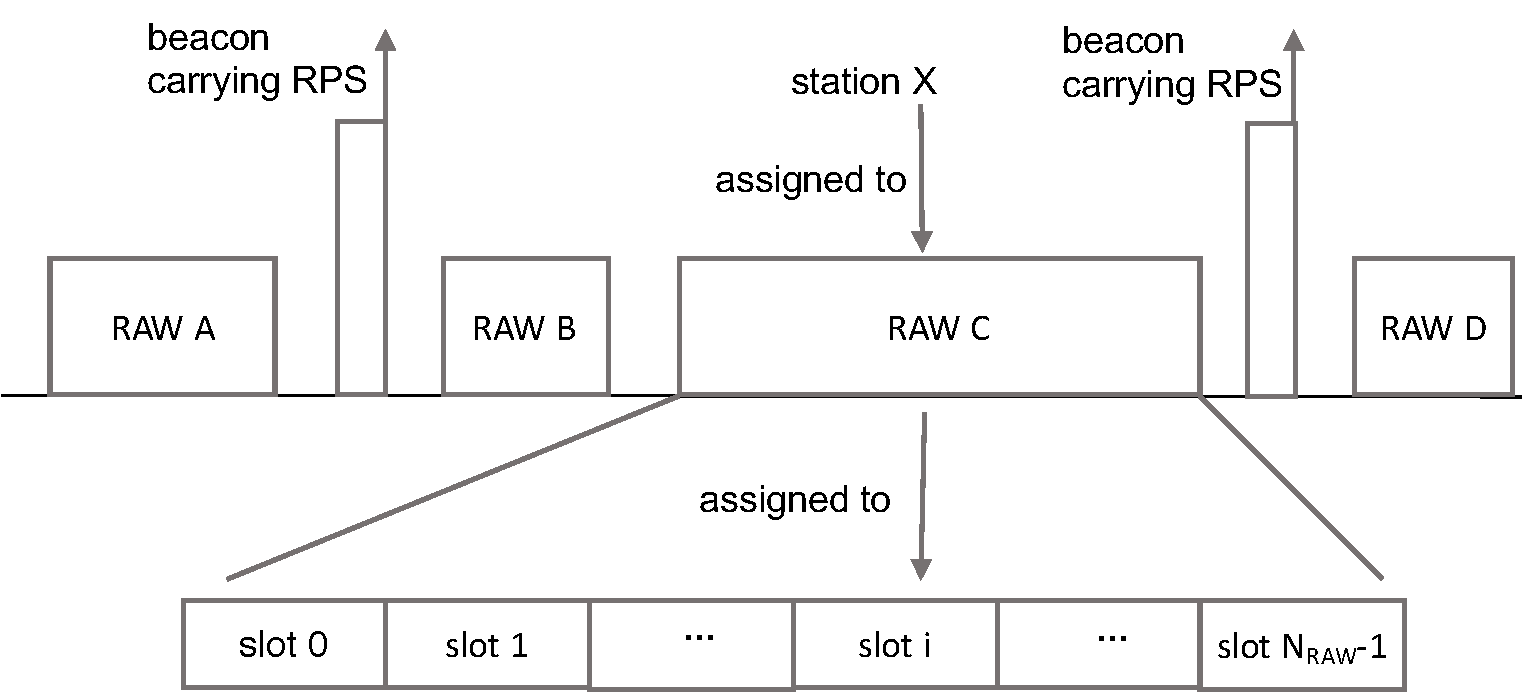
\includegraphics[width=0.8\columnwidth]{figures/raw}
%   \caption{Schematic representation of the \gls{raw} mechanism.\label{fig:RAW}}
% \end{figure}

% The proposed \gls{raw} feature in 802.11ah aims to reduce collisions and improve performance in dense \gls{iot} network
% where hundreds or even thousands of stations are simultaneously contending for channel access.
% It restricts the number of stations that can simultaneously access the channel by splitting them into
% groups and only allowing stations that belong to a certain group to access the channel at specific times.
% Figure \ref{fig:RAW} schematically depicts how RAW works. Specifically, the airtime is split into intervals, some of
% which are assigned to RAW groups, while the others are considered as shared channel airtime and can
% be accessed by all stations. Each interval assigned to a RAW group is preceded by a beacon that carries
% a RAW parameter set (RPS) information element that specifies the stations that belong to the group, as
% well as the interval start time. Moreover, each RAW interval(group) consists of one or more slots, over which
% the stations in the RAW group are split evenly (using round robin assignment). Therefore, the \gls{raw} related parameters include
%  \textit{ number of station assigned to the \gls{raw} groups, number of \gls{raw} groups, duration of each \gls{raw} group}, and  \textit{slot number in each \gls{raw} groups}.
 
% Like the legacy 802.11ah technologies, in physical layer, 802.11ah supports multiple transmission rate represented by \gls{mcs}. As listed in table \ref{tab:wifi-modes},  the number of supported MCS depends on the channel width, for channel width 1 MHz,  MCS 0 $\sim$ MCS 10 are supported with transmission data rate ranging from 150 Kbps to 4 Mbps, and for 2 Mhz, MCS 0 $\sim$ MCS 9 are supported with transmission data rate ranging from 650 Kbps to 7.8 Mbps, more details can be found in \cite{802.11ahStandard}. The stations are allowed to dynamically choose the MCS  for packet transmission to adapt to the conditions of the wireless channel.

% % Table I lists data rates and their MCSs
% % when GI and NSS are 8 us and 1, respectively for 1 and 2 MHz
% % bandwidth.



% As the 802.11 standards do not specify the way of adapting transmission rate, some rate control algorithms have been proposed and used on the real devices to select the appropriate MCS for packet transmission to adapt to the network condition during the past years, for example, Arf \cite{arf1997},  Aarf \cite{aarf2004}, Onoe \cite{Onoe} and Minstrel \cite{minstrel}. The main ideal of these algorithms is to adjust the transmission rate based on the frequency of successful and failed transmission accumulated in the past. 


% \begin{figure}[t]
%   \centering
%   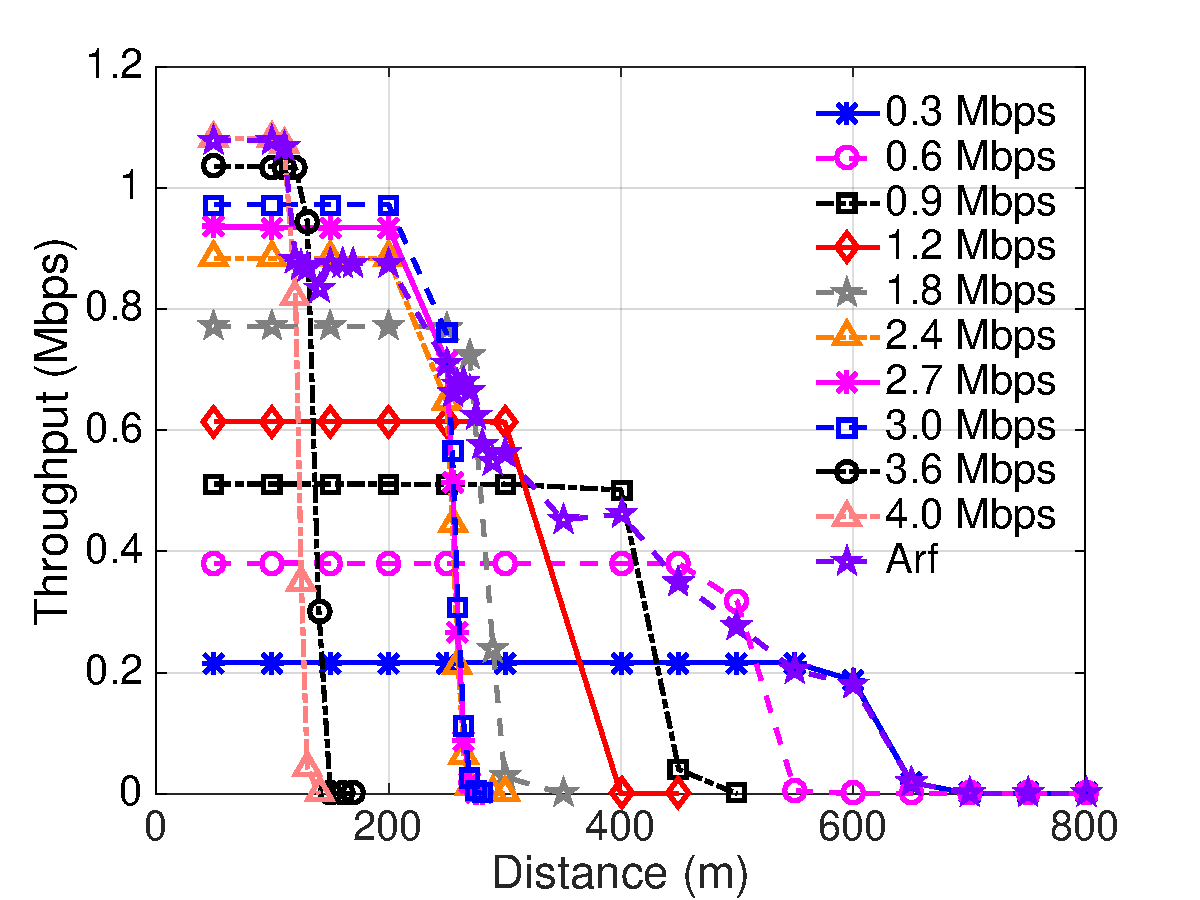
\includegraphics[width=0.45\textwidth]{figures/distance-throughput-512bytes}  \caption{The achievable throughput of each transmission data rate as a function of distance. \label{fig:dist-throughput}}
% \end{figure}

% \begin{figure}[t]
%   \centering
%   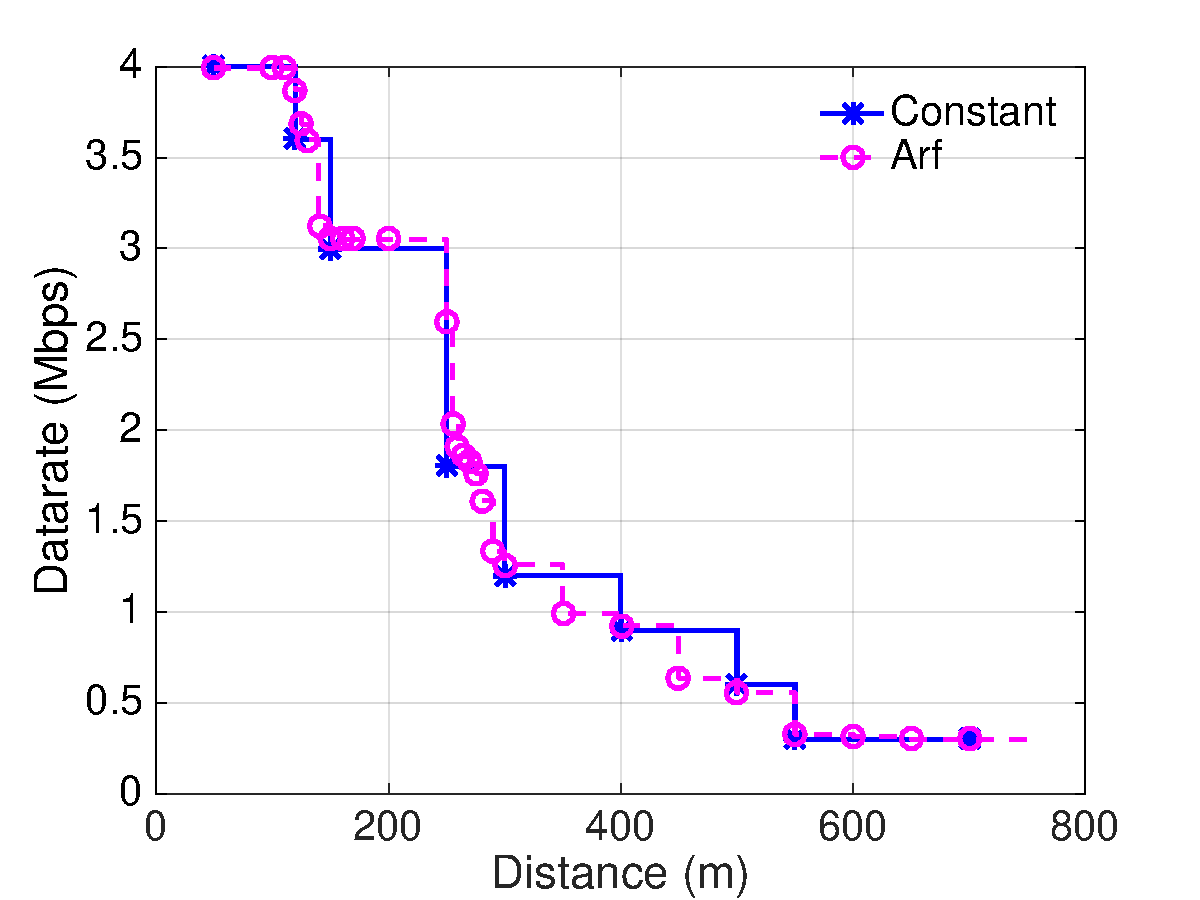
\includegraphics[width=0.45\textwidth]{figures/distance-datarate-512bytes}  \caption{The used transmission data rate for different distance distance. \label{fig:dist-datarate}}
% \end{figure}

% \textcolor{red}{Explain why not use current rca algorithm for modeling}. For the modeling, we use a simpler rate control method, allowing the stations to select the MCS solely based on its distance to the \gls{ap}, i.e., choosing the MCS which can stably achieve the maximal throughput at a certain distance. Figure \ref{fig:dist-throughput} shows the throughput when a station keeps sending packets (512 bytes) to the \gls{ap} at different distance using a certain transmission data rate, and with Arf algorithm as well. Based on the results, figure \ref{fig:dist-datarate} illustrates the rate control method used in the modeling, showing the selected transmission date rate for a certain distance.
% % and the average data rate for a certain distance using arf.
% Although the throughput is achieved with packet size 512 bytes, the same results can be achieved by other packet size as well (not depicted).


% %Rbar \cite{rbar2001},

% % frequency of successful failed transmission accumulated during
% % a fixed invocation period of 1000 ms.

% % In ARF, each sender attempts to use a higher transmission rate after a fixed number of successful transmissions at a given rate and switches back to a lower rate after 1 or 2 consecutive failures. Aarf is an improved version of Arf, we have chosen to adapt this threshold by using a binary exponential backoff When the transmission of the probing packet fails. Onoe is a credit based ragte control algorithm where the value of the credit is determined by the frequency of successful, erroneous and retransmissions accumulated during
% % a fixed invocation period of 1000 ms.

% % Minstrel is based solely on acknowledgement feedback. Consequently, estimates of future success probabilities6 at a given rate
% % are based only on past success ratios at that rate. With a moderate frequency, frames are selected
% % to probe presently unused rates, and feedback from
% % those probe frames maintains the probability estimates
% % for unused rates so that, should the current best rate
% % deteriorate, there is some basis for immediately selecting
% % a more successful rate (Section 5.2)8.

% % In ns-3, multiple rate control algorithms are available, such as for example \textit{ArfWifiManager}, \textit{ConstantRateWifiManager} and \textit{MinstrelWifiManager}. In the original simulator, the IEEE~802.11ah device could only use these algorithms to adapt the \gls{mcs} within the same channel bandwidth. As IEEE~802.11ah supports multiple channel bandwidths (i.e., 1,2,4,8, and 16~MHz), we modified the \textit{WifiRemoteStationManager} class (the parent class of all the rate control algorithms) to allow automatic switching among different channel bandwidths.

% %\item Training methodology (the evaluation scenario used for training)


This sections first introduces the surrogate modeling methodology in general, as well as its integration with the ns-3 network simulator. Subsequently, we describe the IEEE~802.11ah heterogeneous networks used for training. Furthermore, the input and output parameters of the surrogate \gls{raw} model are designed, and steps of training for  the IEEE~802.11ah heterogeneous networks is described. 


\subsection{Surrogate modeling methodology}


\begin{figure*}[t]
  \centering
  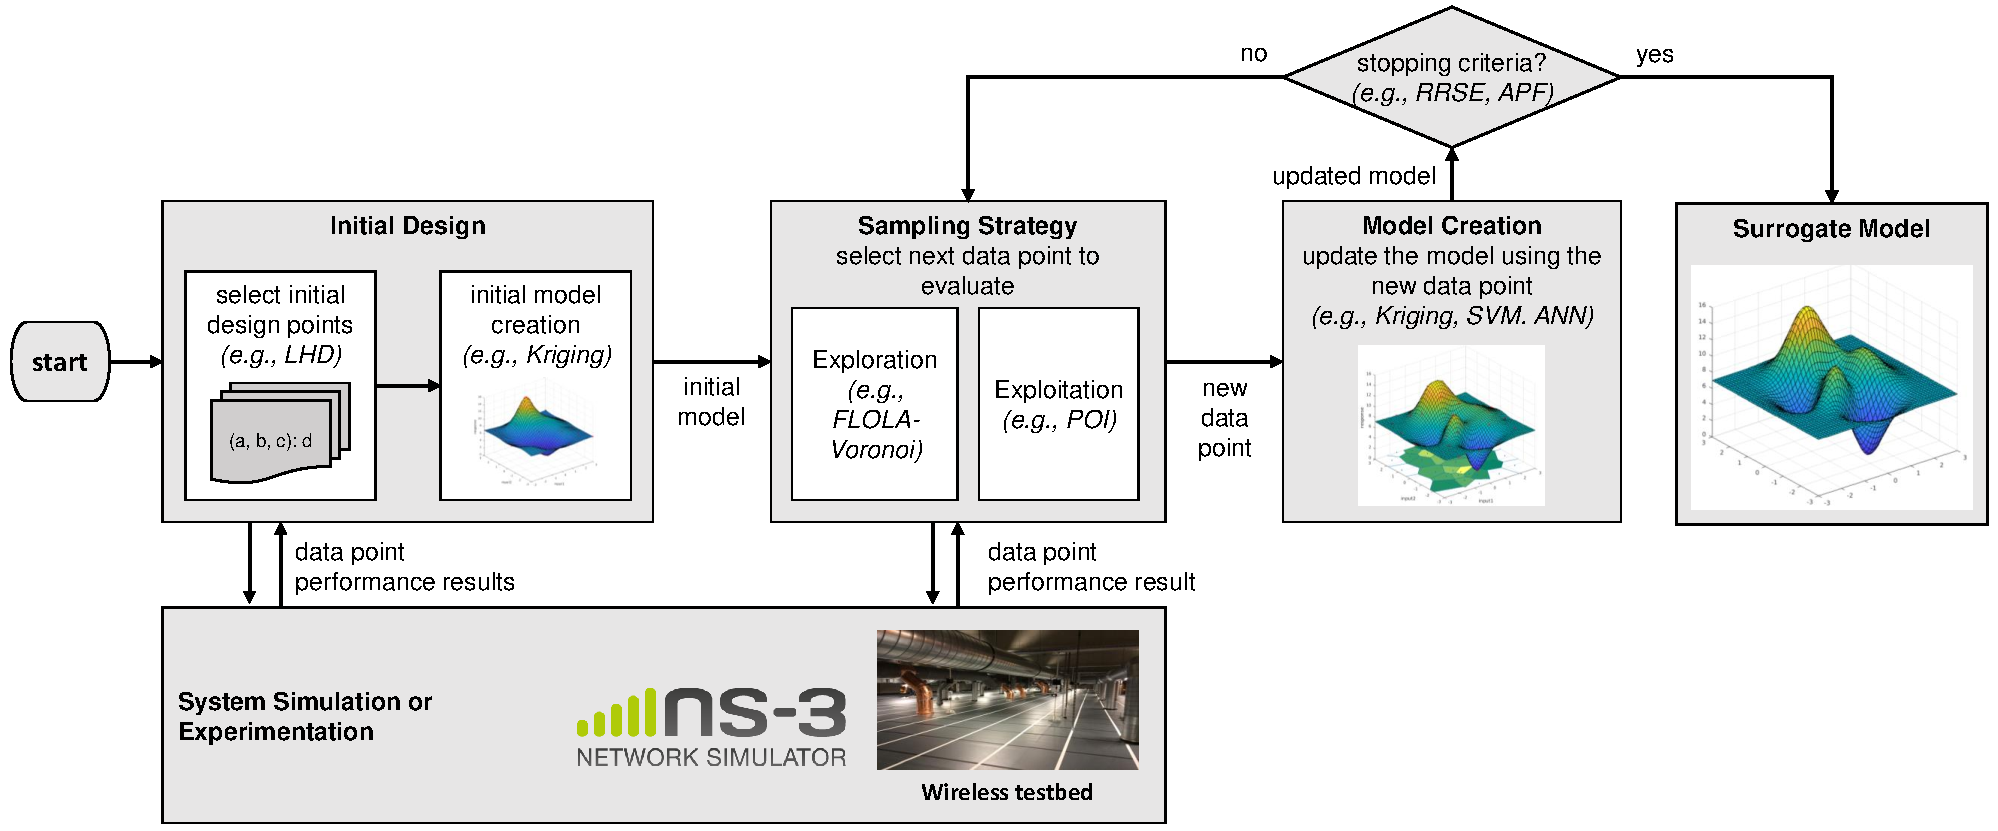
\includegraphics[width=0.75\textwidth]{figures/surrogate_modeling_approach}
  \caption{Surrogate (\gls{raw}) modeling using the ns-3 simulator. \label{fig:sumo-ns3}}
\end{figure*}

 A surrogate model, is an efficient mathematical model that represents the behavior of a complex system such as a circuit, software or wireless network. A surrogate model is trained at design time, using a limited number of input-output sample data points obtained through simulation or real-life experiments. It is especially suited for tasks with a large input space, as an accurate model can be trained based on relatively few input data points. In this paper, we use the \gls{raw} configurations and network conditions as input, and the obtained performance metric (e.g., throughput) 
associated with the input values as output.
As illustrated in Figure \ref{fig:sumo-ns3},  surrogate modeling mainly involves four parts.
 \begin{itemize}
 \item  Initial design. Select initial data points as a first simple design space representation, then build an initial model with the selected initial design points by applying supervised machine learning and regression methods. 
 \item  Sampling strategy. Select a few new sample data points to improve the model if the model's accuracy is not satisfactory.  \item  Model creation. Building an intermediary model together with the existing and newly selected design points. 
 \item  Stopping criteria. Define the stopping criteria, stop the training process once the stopping criteria is satisfied, otherwise, select the new sample data points and update the model. 
 \end{itemize}
  
 The Matlab Surrogate Modeling (SUMO) Toolbox is a flexible framework for accurate global surrogate modeling \cite{SUMOtoolbox2010}, and has already been applied successfully to a very wide range of applications, such as electronic packaging , aerodynamic modeling, process engineering, automotive data modeling, and wireless networks.
 It adopts a microkernel design philosophy with many different plugins available for each step of the surrogate modeling. The behavior of each software component is configurable, and the components can easily be added, removed or replaced by custom implementations. As depicted in Figure \ref{fig:sumo-ns3}, we integrated our previously developed IEEE~802.11ah ns-3 simulation module \cite{WNS32018} into the SUMO toolbox to train the \gls{raw} model. The SUMO toolbox is configured to use the appropriate method in each step in order to create  accurate surrogate model with a limited number of data points. More details are  shown in Section \ref{subs:raw_training}
 %the training process section (i.e., section \ref{subs:raw_training})
 


% \subsection{IEEE~802.11 ah networks and \gls{raw} \label{subsec:80211ah_raw}}



% In this section, we provide an overview of the \gls{raw}, the IEEE~802.11ah network environment and its typical settings on the physical and MAC layers. 
% %A surrogate \gls{raw} model for such network scenarios is subsequently built to accurately predict the performance.


% %simulation environment parameters used during training. 
% %Since \gls{raw} is scalable under uplink traffic, 

% IEEE~802.11ah mainly targets \gls{iot} network scenarios, where sensors (stations) are randomly placed around the AP within a maximum radius, periodically monitor the environment and send the resulting data to a server (via the \gls{ap}). Like the legacy IEEE~802.11 technologies, at the physical layer, IEEE~802.11ah supports multiple transmission data rates represented by the MCSs. The stations are allowed to dynamically choose the MCS for packet transmission to adapt to the conditions of the wireless channel. As listed in Table \ref{tab:wifi-modes}, the number of supported MCSs depends on the channel width. For channel bandwidth 1 MHz,  MCS 0$-$10 are supported with transmission data rates ranging from 150 Kbps to 4 Mbps, and for 2 Mhz, MCS 0$-$9 are supported with transmission data rates ranging from 650 Kbps to 7.8 Mbps, more details can be found in \cite{80211ahStd}. At every beacon interval, the \gls{ap} broadcasts beacon frame carrying a \gls{rps} information element that specifies the \gls{raw} parameter configurations. Stations retrieve such \gls{raw} information from the beacon frame and access the channel only during their assigned \gls{raw} slot. 
% %In order to obtain high performance, there is a need to build a \gls{raw} model that can accurately predict the performance under a variety \gls{raw} parameter values and network conditions.


% The \gls{raw} information is carried in the \gls{rps} element, it specifies the stations belonging to the group, the number of slots, slot format and slot duration count sub-fields, which jointly determine the \gls{raw} slot duration as follows \cite{80211ahStd}: 
% %\textcolor{red}{\cite{80211ahStd}}: 
% \begin{equation} \label{eq:Duration}
% D = 500~\mu{}s + C \times 120~\mu{}s  
% \end{equation}
% where $C$ represents \textit{slot duration count} sub-field, which is either $y = 11$ or $y = 8$ bits long if the slot format sub-field is set to respectively $1$ or $0$. The \textit{number of slots} field is $14-y$ bits long. When $y = 11$, each RAW consists of at most 8 slots and the maximum value of $C$ is $2^{11}-1=2047$, in this case the slot duration is up to $246.14$~ms. Otherwise, each RAW consists of at most 64 slots and the maximum value of $C$ is $2^{8}-1=255$, the slot duration is thus limited to $31.1$~ms. The \gls{raw} group duration is the sum of its slot durations.


\subsection{Training scenarios \label{subsec:training scenarios}}


\begin{figure}[t]
  \centering
  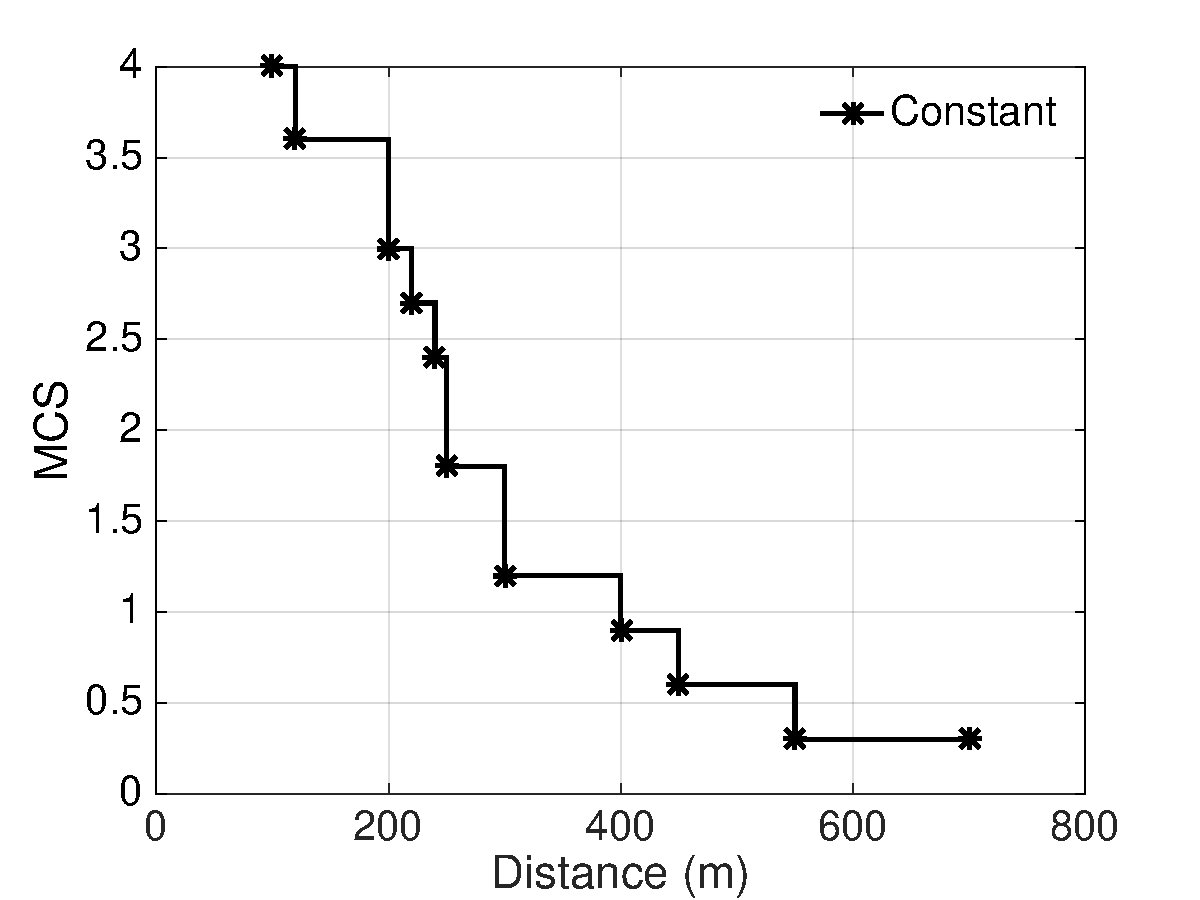
\includegraphics[width=0.45\textwidth]{figures/distance-datarate}  \caption{\gls{mcs} as a function of distance. \label{fig:dist-datarate}}
\end{figure}

Besides \gls{raw}, there are numerous parameters involved in the physical and MAC layer of IEEE~802.11ah networks.
%while we mainly focus on the most commonly used scenarios where
In our experiments, we use the typical parameter settings, 
as shown in Table~\ref{tab:ns3 parameters}. Given the low-power nature of battery powered sensors, the physical layer parameters are configured based on the low-power 802.11ah radio hardware prototype developed by Ba et al.~\cite{Ba2016}, with a transmission power of 0~dBm, a gain of 0~dBi (for both sensor and \gls{ap}), and noise figure of 6.8~dB. With such physical layer setting, the coverage of the networks is up to 500 meters based on the physical layer performance evaluation in \cite{bellekens2017outdoor}. As the \gls{iot} applications have relatively small payload size, packet size is assumed to be between 32 and 512 bytes.


For each experimented scenario, we assume a coverage range to be $[d^-, d^+]  \subseteq [0, 500] $  meters and a packet size range to be $[ps^-, ps^+] \subseteq [32, 512] $ bytes. Each station $s$ randomly and uniformly chooses a value $d_s \in [d^-, d^+]$ as its distance to the \gls{ap}, and an integer value $ps_s \in [ps^-, ps^+]$ as its packet size. Based on its distance to the \gls{ap} $d_s$, the station $s$ uses the corresponding MCS for packet transmission according to the rate control method. Several rate control methods have been proposed and used on the real devices for legacy IEEE~802.11 to select the appropriate MCS for packet transmission, for example, Arf \cite{arf1997},  Aarf \cite{aarf2004}, Onoe \cite{Onoe} and Minstrel \cite{minstrel}. In this paper, We aim to model instantaneous throughput with a single \gls{raw} group (i.e., one beacon interval at most),  \gls{mcs} changes at such a short time slot is are not expected. As such, we allow the stations to select the \gls{mcs} solely based on its distance to the \gls{ap}, i.e., choosing the MCS which can stably achieve the maximal throughput at a certain distance, as shown in Figure \ref{fig:dist-datarate}. The size of the stations' transmit queues is configured to be 10 packets. 
%For training simplicity, we assume each station sends one packet per second, the built model can be further used by the \gls{raw} optimization algorithms, such as \gls{taora} \cite{Sensor2017,Sensys2017},  to calculate \gls{raw} performance under arbitrary data transmission intervals.





% As the \gls{iot} applications have relatively small payload size, we limit the packet size range $[\underline{ps}, \bar{ps}] $ to $[32, 512]$,  choose 500 meters as the maximum distance between stations and the \gls{ap} based on the physical layer performance evaluation in \cite{bellekens2017outdoor}.

%Each experiment runs for 60 seconds of simulated time. As \gls{raw} is configured in each beacon interval of 204.8~ms, the results of every simulated configuration are averaged over 290 beacon intervals, ensuring the generality of the trained model.



%As the RAW optimization algorithm proposed in Section~\ref{sec:algorithm} groups together stations that use the same \gls{mcs}, the model assumes a fixed \gls{mcs}. However, as \gls{raw} performance depends on the \gls{mcs} used, a different model is to be trained for each \gls{mcs} that stations are expected to use. We illustrate this by developing a separate a high-throughput (HT) and low-throughput (LT) model for two different \gls{mcs} parameter sets. This can be trivially extended to other \gls{mcs} values. 


\begin{table}[t]
\centering
\renewcommand{\arraystretch}{1.2}
%\tiny
\caption{\textsc{Simulation parameters used during training}\label{tab:ns3 parameters}}
\begin{tabular}{ll}
\hline
\textbf{PHY parameters}             & \textbf{Value}  \\
\hline
%Frequency (Mhz)                      & 868 \\
TX power (dBm)             & 0    \\
TX/RX gain (dB)                        & 0     \\
Noise Figure (dB)               & 6.8      \\  
%Coding method                  & BCC \\
Propagation model         & Outdoor \\ %, macro~\cite{Hazmi2012} \\
Error rate model               & YansErrorRate \\
\hline
\textbf{MAC parameters}               & \textbf{Value}  \\
\hline
% CWmin                          & 15 \\
% CWmax                          & 1023      \\
%Duration of AIFS (us)\textcolor{red}{change to DIFS}            & 316      \\
Traffic access categories             & \textcolor{black}{ AC\_{BE} } \\
Duration of AIFS ($\mu$s)             & 264      \\
Duration of SIFS ($\mu$s)            & 160      \\
%RTS/CTS                        & not enabled  \\
Beacon interval (ms)           & 204.8 \\
%Cross slot boundary            & Enabled \\
%Rate control algorithm         & constant  \\
Size of transmission queue (packets)  & 10  \\
Packet transmission interval (s)        & 1  \\
Station distribution           & random  \\
%Rate control algorithm                     & XXX \\
%Average payload size (bytes)           & 64   \\
%Topology radius (m)     & 200  \\
\hline
\end{tabular}
\end{table}
 
 
 
\subsection{Parameter design for surrogate \gls{raw} modelling \label{subsec:para_design}}

%\item Input parameters (and motivation and experiments that led to this choice): minimum, maximum, step size, list of parameters, ...
% \begin{itemize}
% \item Add figure(s) to illustrate decisions (cf. Figure Le made in the beginning of the internship)
% \item Average transmission time
% \item RAW parameters.
% \end{itemize}

The goal is to build a surrogate model with a limited number of sample input-output data points, which can accurately predict the performance of a heterogeneous 802.11ah network for the given \gls{raw} settings and network conditions. The input of a data point consists of a set of parameters of a heterogeneous 802.11ah network, and the performance (e.g., throughput) of the associated network is considered as output of the data point. Therefore, a set of parameters should be defined to represent the network conditions and its \gls{raw} configuration. Moreover, the input parameter space needs to be defined, which consists of the minimum and maximum value of each parameter, as well as a step size. The size of input parameters space represents the number of data points of the surrogate model. Among these points, a few of them are selected as sample data points to train the surrogate model, in order to accurately predict the output of the other data points. Therefore, the parameters and their step sizes should be well chosen, leveraging the trade-off between accuracy and training speed. On the one hand, a small number of parameters and large step sizes lead to a small design space, which needs less training time but poorly characterizes the system. On the other hand, a large number of parameters and small step sizes result in a big design space, which can more accurately characterize the system but needs more training time. As for the output parameter of the model, it should be able to represent the performance metrics (e.g., throughput, energy consumption and latency) with the given input parameters. To simplify the explanation, we focus on throughput as an output metric.



\subsubsection{\gls{raw} parameter design \label{subsec:raw_para_design}}

As mentioned in Section \ref{subsec:80211ah_raw}, the related parameters of a \gls{raw} group $r$ are, number of station assigned to the \gls{raw} groups $n_r$, duration of the \gls{raw} group $d_r$, and slot number in the \gls{raw} group $s_r$. In our previous work \cite{wowmom2018}, we selected the appropriate range and step size for each \gls{raw} parameter, which leads to high model accuracy and only a limited number of training data points. Therefore, in this paper, we use the same \gls{raw} parameter values. A minimum value of $60$ and maximum value of $400$ stations per group $n_r$ were deemed to cover all possible traffic conditions, $d_r$ is varied between $40960$~$\mu$s and $204800$~$\mu$s, and  $s_r$ is between 1 and 50. This results in $2.3 \times 10^7$ possible combinations, which is too high to train the model in a feasible amount of time. Thus, a good step
size for each of the three \gls{raw} parameters is chosen, leveraging the trade-off between accuracy and training speed.
For $n_r$ and $s_r$ a step size of 5 was selected, and $s_r$ takes on values from the set $\left\{1, 5, 10, ..., 50\right\}$. As such, $25047$ combinations are generated with \gls{raw} parameters, and the total number of data points of the input space is $25047 \times m$, where $m$ represents the number of combinations from the network condition parameters.

\subsubsection{Network condition parameter design \label{subsec:network_para_design}}

As in the IEEE~802.11ah network environment, the typical settings are used for  some parameters (cf. Table \ref{tab:ns3 parameters}), the remaining variables are the  packet size  range $[ps^-, ps^+]$ and coverage range $[d^-, d^+]$, which leads to a variety of heterogeneous networks. It seems straightforward to use these four parameters as the input parameters of model, representing the networks conditions. However, this would result in a huge input design space, significantly increase the required training data points and therefore slowing the training speed. According to the training scenarios, the $d^-$ and $d^+$ is between 0 and 500 meters with $d^- \leq d^+$, the $ps^-$ and $ps^+$ is between 0 and 512 bytes with $ps^- \leq ps^+$. With step size 1, the coverage range and packet size range  results in 125751 and 115921 combinations respectively, and $m = 1.4 \times 10^{10} $ combinations in total. Therefore, the total number of data points of the input space is $25047 \times m = 3.5 \times  10^{14}$. With a large step size, for instance, 100 for  the coverage and 120 for the packet size, the input space still has $7.89 \times  10^{6}$ data points. Both cases results in design space that is too big to achieve feasible convergence. Therefore, as MCS (equivalent to data rate and derived from distance) and packet size can jointly determine the transmission time of a packet, we decide to use average packet transmission time $T_x$ of all stations as the input parameter representing network conditions, leveraging the trade-off between accuracy and training speed (equivalent to input design space). The remaining of this section elaborates the highly reduced input design space, including the distribution of average transmission time $T_x$ among the IEEE~80.211ah network scenarios, and its minimum,  maximum and step values. The accuracy is detailed in Section \ref{subsubsec:txselection}.

%and packet receiving rate as the output parameter of the mode. 
%The reason is detailed in the reminder of this section.

%Hereby we present the distribution of average transmission time $\hat{t}_p$ among the IEEE~80.211ah network scenarios, and define its minimum and maximum value as an input parameter of the surrogate model. 
Figure \ref{fig:tx-hist} depicts the distribution of average transmission time $T_x$ of the training scenarios. The figure is derived from the simulation results of a broad range of networks which have different coverage and packet size ranges. The $d^-$ and $d^+$ parameters are selected from [\textit{min}:\textit{step}:\textit{max}]=[0:10:500] meters, and the $ps^-$ and $ps^+$ belong to  [\textit{min}:\textit{step}:\textit{max}]=[32:32:512] bytes. Therefore, the combination of coverage and packet size range leads to 180336 different 802.11ah networks. We calculate the average packet transmission time across all stations in each network, and count how many times a certain average transmission time occurs among the 180336 802.11ah networks. The results in Figure \ref{fig:tx-hist} shows the average transmission time in the range of [1200 1500] $\mu$s occurs the most (24660 times),  and the average transmission time is mainly between 1000 $\mu$s and 5000 $\mu$ (around 90\% of all experiments). Therefore,  when average transmission time is considered as an input parameter of the model, 1000 and 5000 $\mu$s can be used as its minimum and maximum value for the training. A step size of 250 is selected, leading to $m = 17$ different values for average transmission time.
Therefore, using average transmission time results in a design space with only $25047 \times m = 425799$ data points, from which samples are drawn during the training.
It is only $1.2 \times 10^{-7} \%$ of all data points (i.e., $3.5 \times 10^{14}$) in the design space in which $d^-$, $d^+$, $ps^-$ and $ps^+$ are used as input parameters to represent the network.

% much less than $3.5 \times 10^{14}$ data points caused by using $d^-$, $d^+$, $ps^-$ and $ps^+$ as input parameters to represent the network.
%\textcolor{red}{The surrogate model can interpolate the results for data points outside the input parameter space}.


%Results for data points outside the input parameter space are obtained via linear interpolation of the two nearest data points included in the model.
 
 %\textcolor{red}{todo, explain the huge space caused by the four parameters.}

%%[0, 500], [32, 512]
%%step size 1
%% for [0, 500], num = 501 + 500 + ... + 1 = 125751
%% for [32, 512], num = 481 + 480 + ... + 1 = 115921
%% total, 125751 * 115921 = 14577181671
%% with raw, total, 14577181671 * 25047 = 365114669313537

%% step size 100/120
%% for [0, 500], 21
%% for [32, 512], 15
%% total, 315
%% with raw, total, 315 * 25047 = 7889805
 \subsubsection{Output parameter design \label{subsec:output_para_design}}

 As an average transmission time can consist of a variety of packet size ranges that can affect the throughput, the successfully packet receiving rate (i.e., number of received packets per seconds) is used as the metric of performance. The throughput can be subsequently calculated
together with the packet size range for a specific network scenario.
 

 
 
% As small average transmission time, for example transmission time $1000$ \textit{us}, has relative short distance  and packet size, leading to small variance on the packet rate. While for large transmission time, stations have longer distance to the \gls{ap} and larger packet size, therefore, the packet rate has larger variance.

% with average transmission time no more than 3000 us have the similar performance regardless of the coverage and packet size range. However, with larger average transmission time, the results are quite different,  in this case, the average transmission time can not be used to represent the network, and therefore, can not be used as an input parameter to train the model. As such, we limit the average transmission time to between 1000 us and 3000 us. We choose 250 as the step size of  $\hat{t}_p$.



% In probability theory and statistics, the coefficient of variation (CV), also known as relative standard deviation (RSD), is a standardized measure of dispersion of a probability distribution or frequency distribution.

Therefore, the surrogate model can be represented as a function  $\mathcal{F}$ :
\begin{equation} \label{eq:raw_model}
p_r = \mathcal{F}(n_r, d_r, s_r, T_x) 
\end{equation}
Where $p_r$ represents the packet receiving rate. It aims to predict the performance of a heterogeneous 802.11ah network with average packet transmission time $T_x$, for a given RAW group $r$ with duration $d_r$, consisting of $s_r$ slots, and with $n_r$ stations assigned to it. The definition of the input parameters are listed in Table \ref{tab:sumo parameters}.

%\subsection{The selection of parameter average packet transmission time \label{subsubsec:txselection}}

\subsection{Network condition parameter analysis \label{subsubsec:txselection}}

In this section, we demonstrate that the average transmission time 
%and packet receiving rate 
is a proper input parameter for the model, as it can accurately represent the network conditions with highly reduced design space size. As the size of design space has been discussed in section \ref{subsec:network_para_design}, this section focus on the accurate representativeness. The accurate representativeness lies on that, networks with the same average transmission time have small variance in the behaviour, i.e., similar packet receiving rate, in order to accurately predict one for the other. Since the model is mainly used for optimization, we are more interested in the large values and high \gls{pdr}.
\gls{pdr} is defined as the ratio between the number sent packets, and number of received packets predicated by the model. The large values signify higher throughput and better performance, and high \gls{pdr} indicates lower packet loss. The \gls{cov}, also known as relative standard deviation, is a measure of variation or dispersion of a set of data values, it is calculated by dividing the standard deviation of a series of values by the average of the values. In this section, the \gls{cov} is used as the criterion to evaluate the variance of the output (i.e., packet receiving rate)  of networks with the same average transmission time $T_x$ but different coverage and packet size ranges. As Figure \ref{fig:tx-hist} shows, there are a large number of coverage and packet size ranges that can lead to the same average transmission time. 


%\gls{cov} is a measure of variation or dispersion of a set of data values, it is calculated by dividing the standard deviation of a series of values by the average of the values.


%it is vital that the networks with the same average transmission time have the similar behaviour, i.e., similar packet receiving rate, in order to accurately predict one for the other.



%The CV or RSD is widely used in analytical chemistry to express the precision and repeatability of an assay. 

%As an average transmission time can consist of a variety of packet size range that can affect the throughput, the successfully packet receiving rate  (i.e., number of packet per seconds) is used as the metric of the performance. The throughput can be subsequently calculated together with the packet size range for a specific network scenario.

%In order to proof the viability of using average transmission time as the input parameter representing the network conditions, we compare the performance ( i.e., packet receiving rate) of different coverage and packet size ranges, which all results in the same average transmission time $T_x$. 




The variance is evaluated under different packet receiving rate and \gls{raw} slot load ratios. The \gls{raw} slot load ratio is defined as the ratio between the required transmission time of the 
packets that are allowed to transit in a \gls{raw} group, and duration of the \gls{raw} group. Its definition is as follows:
 \\
\begin{equation}
\mathcal{L}_{r} = \frac {n_r \times TXOP} {d_r \times \mathcal{T}_s}. 
\end{equation}
\begin{equation}
TXOP = T_x + T_{SIFS} +  T_{ACK}
\end{equation}
Where $TXOP$ indicate the time including data packet transmission time $T_x$, a SIFS time (160 $\mu$s) and the ACK transmission time (1000 $\mu$s). $\mathcal{T}_s$ represents the packet sending interval of a station. A large value means a high input traffic load, and vice versa. The network is under overloaded traffic condition when slot load ratio is larger than 1.
%The minimal slot traffic load which can cause performance discrepancy is denoted as $\mathcal{L}_r^max$, in order to apply the model to the extended design space, the slot traffic load needs to be no larger than the $\mathcal{L}_r^max$. For transmission time $1000$ and $5000$ \textit{us}, the  $\mathcal{L}_r^max$ are \textcolor{red}{xx} and \textcolor{red}{xx}, respectively.
In the evaluation, 500 design points for each average transmission times (i.e., 1000, 2000, 3000, 4000 and 5000 $\mu$s) are randomly selected, 
consisting of 5 different \gls{raw} slot load ratio (i.e., 0.4, 0.6, 0.8, 1.0, 1.6). Each data point has four input parameters, i.e., number of station, number of slot, \gls{raw} duration, and average transmission time. The simulation runs 10 times for each data point. During each simulation, the simulator randomly selects a different coverage and packet size range satisfying the required average transmission time. After simulation, the \gls{cov} of each data point's output (i.e., packet receiving rate) is calculated. Subsequently, for each average transmission time, the \gls{cov} is averaged, among the data points with the same packet receiving rate and \gls{raw} slot load ratio respectively. The final results are shown in Figure \ref{fig:tx-diff-Prate} and \ref{fig:tx-diff-load}, each includes the results of both all data points and only the data points with \gls{pdr} larger than 80\%.
%It turns out, the performance variability of the network \textcolor{red}{ (data point) is relevant} to  average transmission time, packet receiving rate, and \gls{raw} slot load ratio.



Figure \ref{fig:tx-diff-Prate-all} shows that, small packet receiving rate (i.e., less than 60) can result in quite high performance discrepancy, with \gls{cov} 1.009 and 2.08 for average transmission time 1000 $\mu$s and 5000 $\mu$s respectively. For the larger packet receiving rate, the \gls{cov} is around 0.25 for average transmission time 4000 $\mu$s and 5000 $\mu$s, the variance is still high. However, when focus on the data points with \gls{pdr} larger than 80\%, the \gls{cov} is significantly reduced, as depicted in Figure \ref{fig:tx-diff-Prate-08}. Moreover, the smaller average transmission time results in less variability, while the larger average transmission time leads to more variability. For example, the \gls{cov} is at most 0.02, between 0.02 and 0.07, for average transmission time 1000 and 2000 $\mu$s. While for average transmission time 5000 $\mu$s, the \gls{cov} ranges from 0.1 to 0.16. It should be noted that, the maximum achievable packet receiving rate decreases as the average transmission time increases, since more time is needed for one packet transmission.
%The high performance discrepancy for small packet receiving rate make sense, as a small value more easily leads to a large discrepancy. 
% the smaller average transmission time results in less variability, while the larger average transmission time leads to more variability. Moreover, a small packet receiving rate (i.e., less than 60) results in quite high performance discrepancy, with \gls{cov} 1.009 and 2.08 for average transmission time 1000 $\mu$s and 5000 $\mu$s respectively. For larger packet receiving rates, the performance remains stable, the \gls{cov} is less than 0.03 and around 0.06 for average transmission time 1000 and 2000 us, around 0.12 and 0.15 for average transmission 3000 and 4000 us, and 0.25 for average transmission time 5000 us. The high performance discrepancy for small packet receiving rate make sense, as a small value more easily leads to a large discrepancy. It should be noted that, the maximum achievable packet receiving rate decreases as the average transmission time increases, since more time is needed for one packet transmission.
Figure \ref{fig:tx-diff-load-all} again demonstrates that, average transmission time has a significant impact on the performance discrepancy. Furthermore, it reveals that the performance variation increases with larger \gls{raw} slot load. However, except for average transmission time 1000 $\mu$s, the \gls{cov} is quit high (above 0.2) in most cases. By only focusing on the data points with \gls{pdr} larger than 80\%, the \gls{cov} can be significantly reduced, as depicted in Figure \ref{fig:tx-diff-load-08}.
For example, the \gls{cov} is 0.001 and 0.02 for \gls{raw} slot load ratio 0.4 and 1.0 when average transmission time is 1000 $\mu$s. For average transmission time 3000 $\mu$s, The \gls{cov} ranges from 0.05 to 0.1,  from 0.1 to 0.16, for  average transmission time 3000 and 5000  $\mu$s, respectively. 



 %The higher \gls{raw} slot load ratio means more fierce condition, 

%Figure \ref{fig:tx-diff-load}, only the data points whose packet receiving rate is more than 60 are depicted. The result again demonstrates that, average transmission time has a significant impact on the performance discrepancy. Furthermore, it reveals that the performance variation increases with larger \gls{raw} slot load. 
% For example, for average transmission time 1000 $\mu$s, the \gls{cov} is 0.009 and 0.05 for \gls{raw} slot load ratio 0.4 and 1.6 when average transmission time is 1000 $\mu$s. 
% %For average transmission time 3000 us, the \gls{cov} is 0.05 and 0.15 for \gls{raw} slot ratio 0.4 and 0.8, increase to 0.18 for overloaded traffic (i.e, \gls{raw} slot ratio 1.6).  
% While for average transmission time 5000 $\mu$s, the \gls{cov} is relative large, ranging from 0.18 to 0.41 when \gls{raw} slot ratio increases from 0.6 to 1.6. \todo{reason}
% The higher \gls{raw} slot load ratio means more fierce condition, 



 
Since the trained \gls{raw} model is mainly used for performance optimization, mainly the data points with large packet receiving rate are and high \gls{pdr} are our focus, 
based on the results shown in Figure \ref{fig:tx-diff-Prate} and \ref{fig:tx-diff-load}, we can conclude that  average transmission time is able to represent the conditions of network. Therefore, in this paper, we use the average transmission time as a input parameter for the training.
 
The fact that the performance variance are affected by the factors, including packet receiving rate, \gls{raw} slot ratio, \gls{pdr} and average transmission time, can be explained as follows. 
%  The large \gls{cov} exists for small packet receiving rate is due to the fact that a small values is more easily leads to a large variance. As the networks (i.e., data points) have different input parameters, even the networks sharing the same input parameters may have different coverage and packet size ranges, there are different saturated levels for these networks. With larger \gls{raw} slot ratio, the channel contention is more fierce, therefore, the performance of different networks are more discrepancy. Data points with higher \gls{pdr} implies that, they have proper \gls{raw} configurations that mitigate the channel contention, leading to higher saturated levels. Therefore, less performance discrepancy among different networks is obtained. 
 \begin{itemize}
 \item \textbf{Packet receiving rate} \\
 The large \gls{cov} exists for small packet receiving rate is due to the fact that a small values is more easily leads to a large variance.
 \item  \textbf{\gls{raw} slot load ratio} \\
 As the networks (i.e., data points) have different input parameters, even the networks sharing the same input parameters may have different coverage and packet size ranges, there are different saturated levels for these networks. With larger \gls{raw} slot ratio, the channel contention is more fierce, therefore, the performance of different networks are more discrepancy.
 \item \textbf{\gls{pdr}} \\
 Data points with higher \gls{pdr} implies that, they have proper \gls{raw} configurations that mitigate the channel contention, leading to higher saturated levels. Therefore, less performance discrepancy among different networks is obtained.
 \item \textbf{Average transmission time} \\
 For each network with average transmission time $T_x$, Figure \ref{fig:tx-std-dist} depicts its standard deviation of packet transmission time across all stations. It shows, for networks with a same and lager average transmission time, there is a higher chance that these networks have different packet transmission time distribution. Such difference can result in performance discrepancy when packet collision happens, as the airtime wasted by collision and required by re-transmission depends on the transmission time of collide packets.
  \end{itemize}


%  average transmission time can represent the conditions of network, which has small average transmission time, large packet receiving rate and non-overloaded traffic. In this paper, we use the average transmission time as a input parameter for the training, due to the following three reasons. First of all, the trained \gls{raw} model is mainly used for performance optimization, mainly the data points with large packet receiving rate are interesting. Second, overload traffic is not common in realistic scenarios, we only need to focus on the non-overloaded traffic scenarios. Last but not least, as mentioned in section \ref{subsec:network_para_design}, compare to parameters {${d^-}$, ${d^+}$, ${ps^-}$, ${ps+}$}, average transmission time $\hat{p_p}$ lead to an input design space with only xx data points. Therefore, there is a trade-off between the accuracy and training speed. \textcolor{red}{Tx 5000 us results in high performance discrepancy, should we mentioned the model is not suitable for Tx 5000?}. During the training, network scenarios with the same average transmission time use a fixed coverage range and packet size range. 

% explanation
%The performance discrepancy of an average transmission time for different coverage and packet size ranges is mainly caused by the propagation loss, capture effect. As the location and packet size distribution among stations is different. As small average transmission time, for example transmission time $1000$ us, has relative short distance  and packet size, leading to small variance on the packet rate. While for large transmission time, stations have longer distance to the \gls{ap} and larger packet size, therefore, the packet rate has larger variance. \todo{update the explanation.}


% To build the surrogate model, the input parameter space needs to be defined. It consists of the minimum and maximum value of each parameter, as well as a step size. The minimum and maximum can be determined based on expert knowledge of \gls{raw} performance, as well as legal values defined by the IEEE~802.11ah standard. The range of the number of stations $n_r$ in a \gls{raw} group should span from low to high traffic conditions, so the trained model gives accurate results independent of the density. From our previous studies on \gls{raw} performance~\cite{wowmom2018}, for MCS with bandwidth 1 MHz and packet size less than 512 bytes, a minimum value of $60$ and maximum value of $400$ stations per group were deemed to cover all possible traffic conditions. The number of slots $s_r$ is bound between $1$ and $64$, as per the IEEE standard. However, a very high number of slots leaves not enough time within a slot to successfully transmit a packet. As such, we limit $s_r$ between 1 and 50. The RAW group duration should be large enough to allow at least 1 packet is successfully sent in each \gls{raw} slot, and at most equal to the duration of the beacon intervals. As such, by taking the \gls{raw} slot number into account, $d_r$ is varied between $40960$~$\mu$s and $204800$~$\mu$s.


% 
%Several aspects are involved:
%1, the same average transmission time can results in different output.
%2, the same network (coverage and packet size range) can have quite different outputs for different randomization seeds.
%3, load ratio also play an ratio, the performance difference among networks with same average transmission time increases when load ratio increase.


% The actual step size of $n_r$, $s_r$ and $\hat{t}_p$ is $1$, as they are integer variables. The parameter $d_r$ has a step size of $120$~$\mu$s, as defined in the 802.11ah standard. This results in a total input space of \textcolor{red}{$2.3 \times 10^7$} possible data points. This is too high to properly train the model in a feasible amount of time. To alleviate this, we experimentally determined a good step size for each of the parameters, leveraging the trade-off between accuracy and training speed. For $n_r$ and $s_r$ a step size of 5 was selected, 250 is choose as the step size of  $\hat{t}_p$. It was found that the \gls{raw} duration $d_r$ has a high sensitivity. As such, a small value of $5120$~$\mu$s was chosen as its step size. This results in a significantly reduced input space of \textcolor{red}{$25047$} data points. Table~\ref{tab:sumo parameters} summarizes the selected input parameter space. Note that a slot count $s_r$ equal to $0$ is not legal, and $s_r$ therefore takes on values from the set $\left\{1, 5, 10, ..., 50\right\}$. 


%Results for data points outside the reduced input parameter space are obtained via linear interpolation of the two nearest data points included in the model.

\begin{figure}[t]
  \centering
  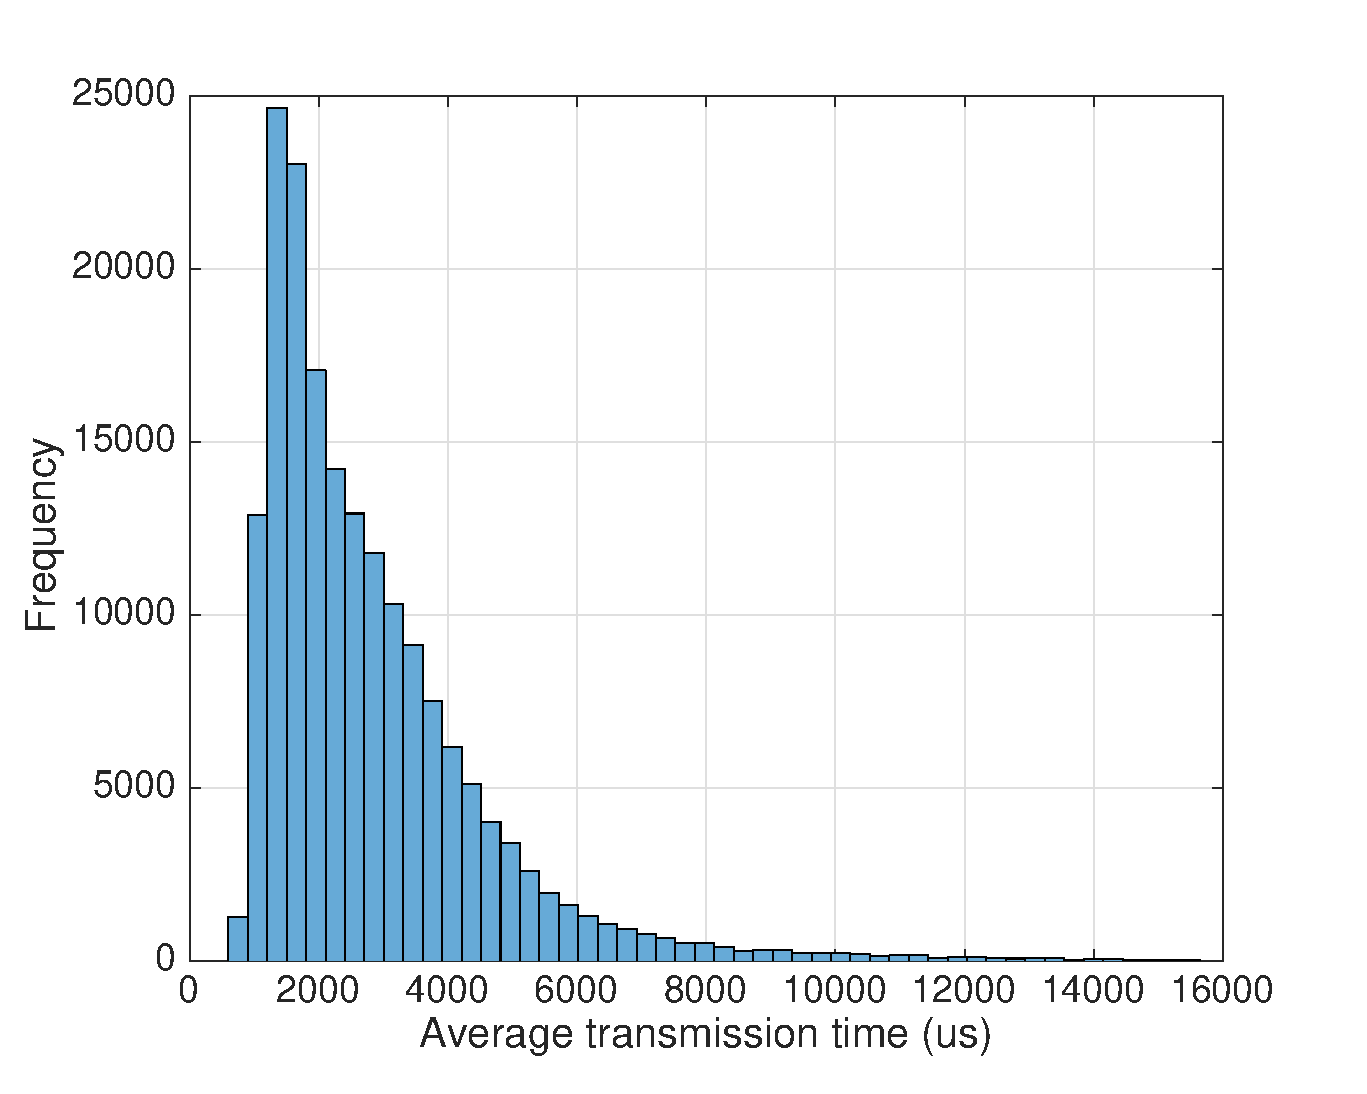
\includegraphics[width=0.75\columnwidth]{figures/histTx}
  \caption{Distribution of average transmission time of 802.11ah networks supporting different coverage and packet size ranges. \label{fig:tx-hist}}
\end{figure}


% \begin{figure}
%   \centering
%   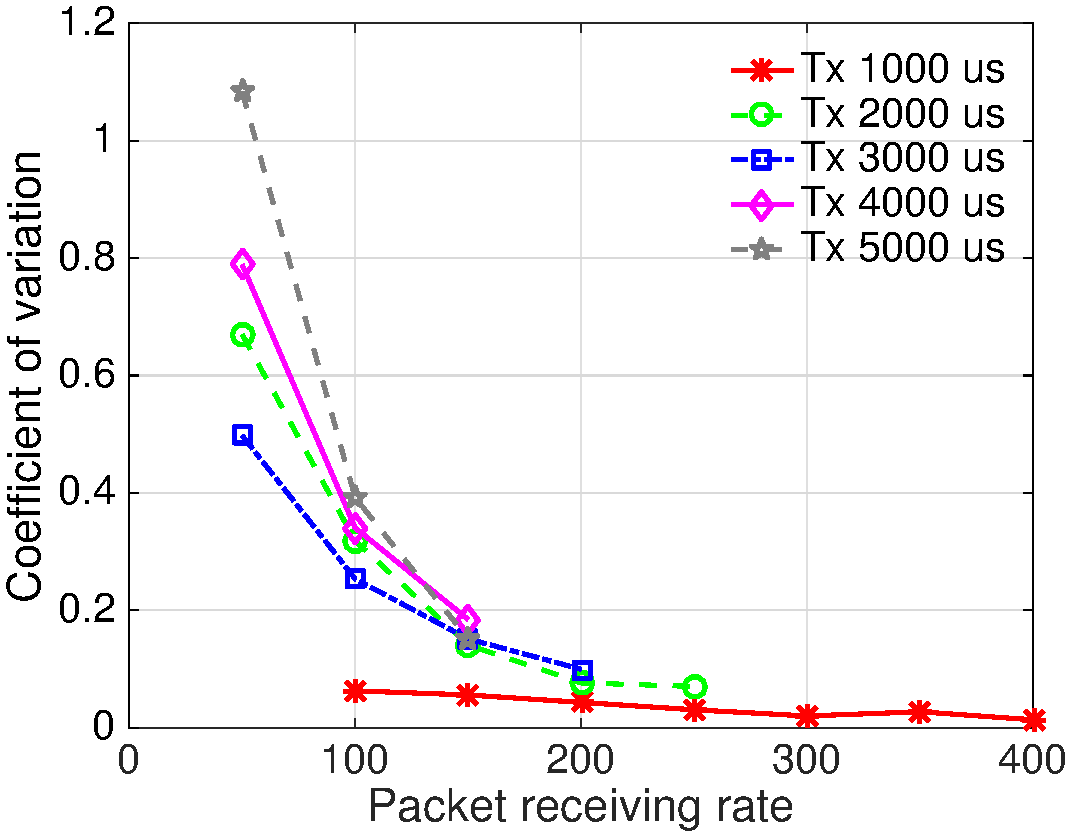
\includegraphics[width=0.75\columnwidth]{figures/avg_result_Prate_tx_ratio3_20}
%   \caption{\textcolor{red}{To be updated}. \label{fig:tx-diff}}
% \end{figure}


% \begin{figure}[t]
%   \centering
%   % 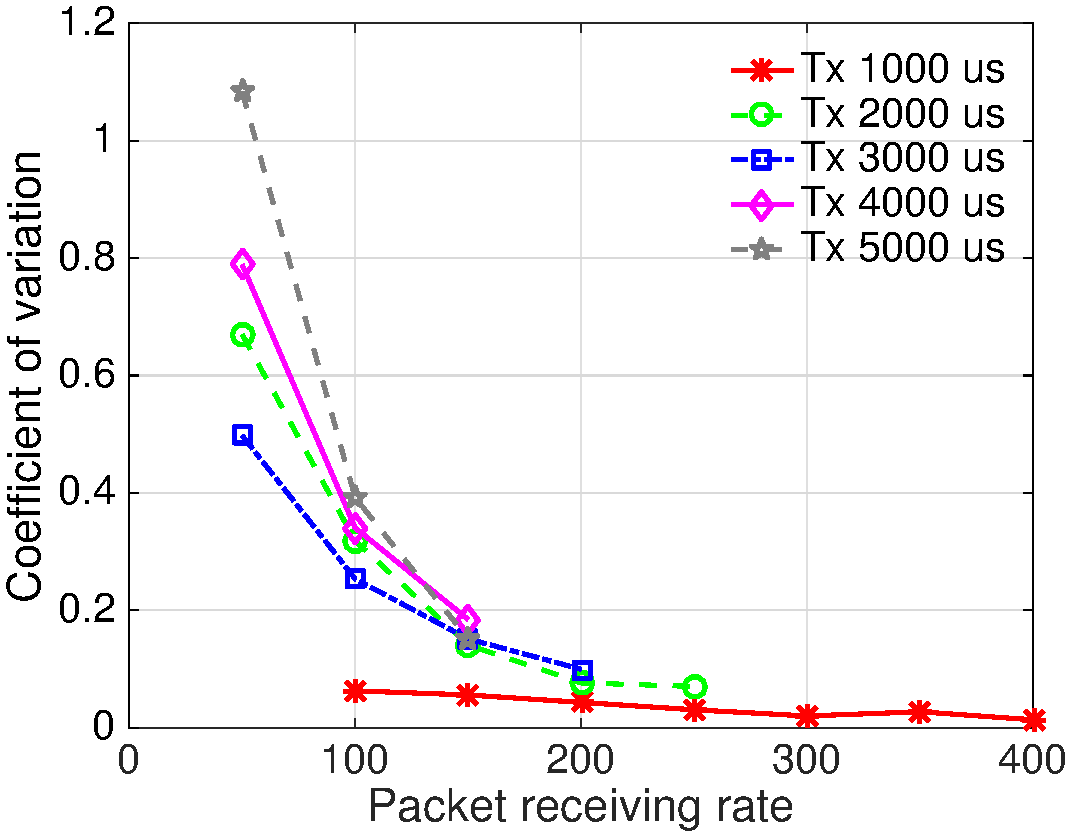
\includegraphics[width=0.75\columnwidth]{figures/avg_result_Prate_tx_ratio3_20.pdf}
% %      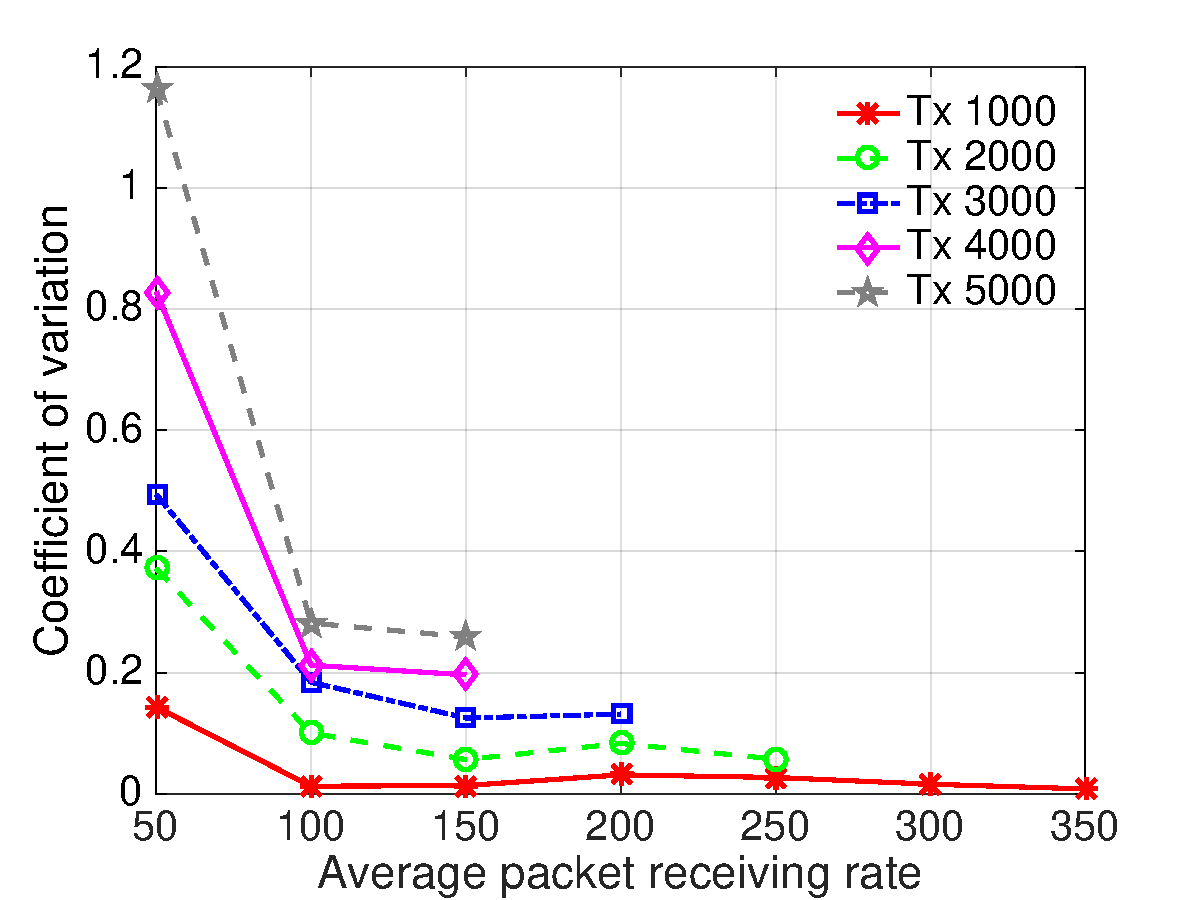
\includegraphics[width=0.75\columnwidth]{figures/avg_result_Prate_tx.pdf}
%   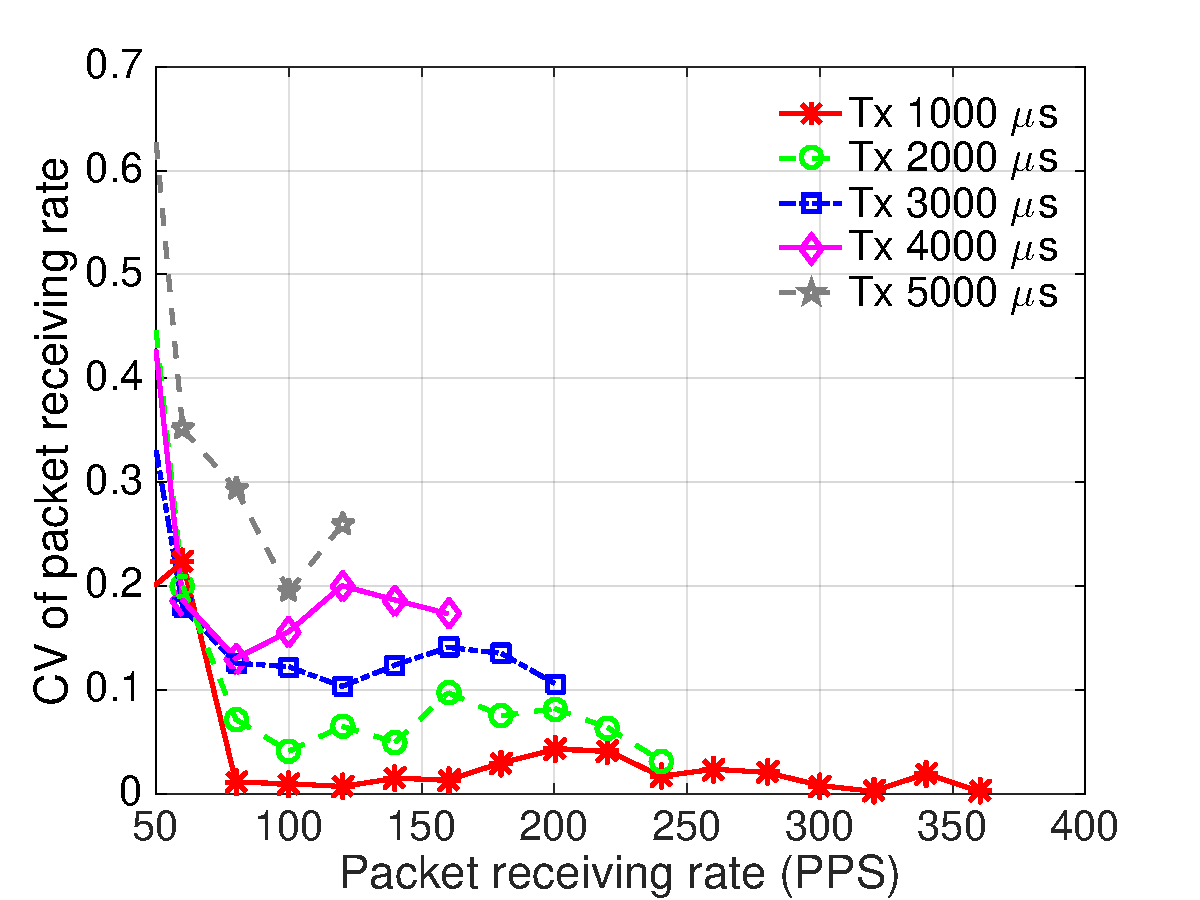
\includegraphics[width=0.75\columnwidth]{figures/new_load_avg_result_Prate_tx_all.pdf}
%     \caption{  \gls{cov} of packet receiving rate as a function of packet receiving rate for each different average transmission time %consisting of different coverage and packet size ranges.
%     \label{fig:tx-diff-Prate}}
% \end{figure}


\begin{figure*}[t]
    \centering
    \subfloat[All data points  \label{fig:tx-diff-Prate-all}]{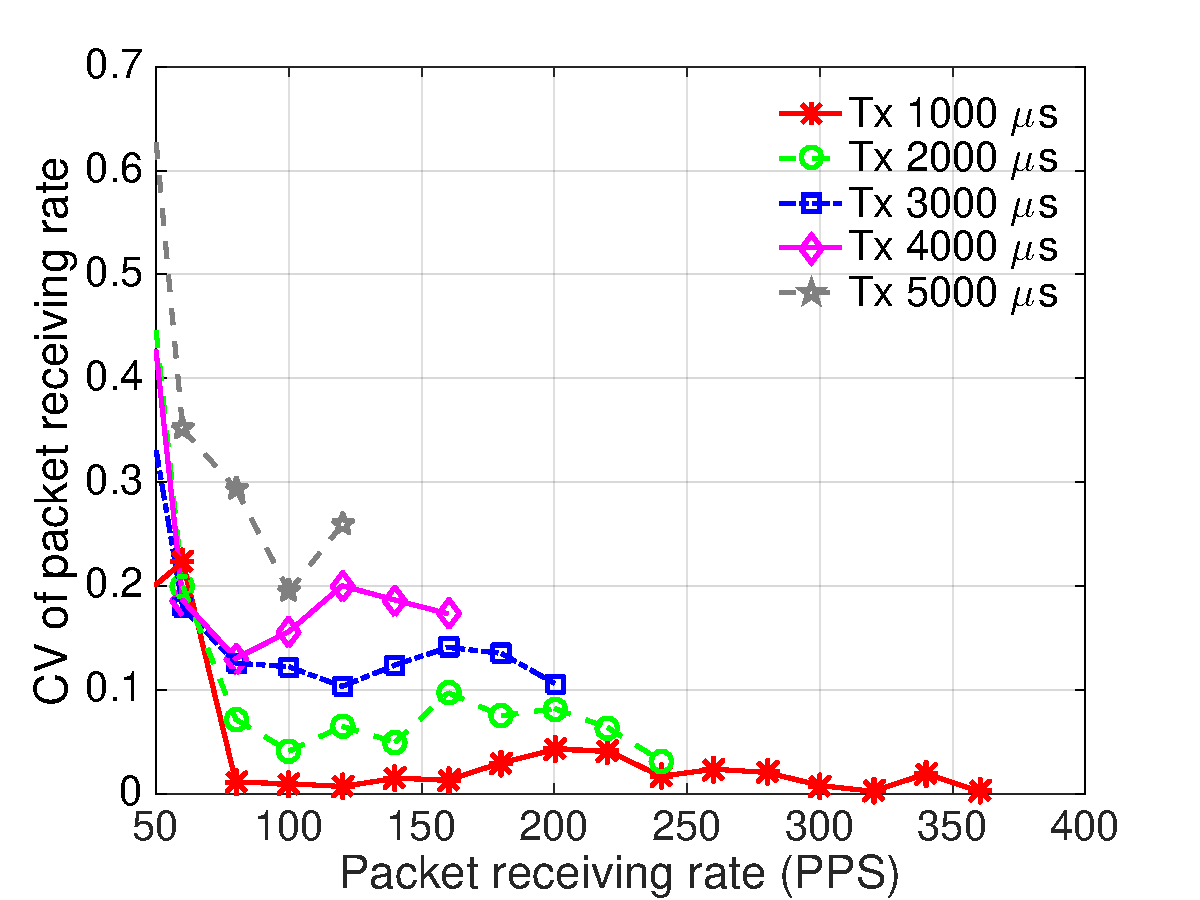
\includegraphics[width=0.45\textwidth]{figures/new_load_avg_result_Prate_tx_all}} 
    \subfloat[data points with \gls{pdr} more than 80\% \label{fig:tx-diff-Prate-08}]{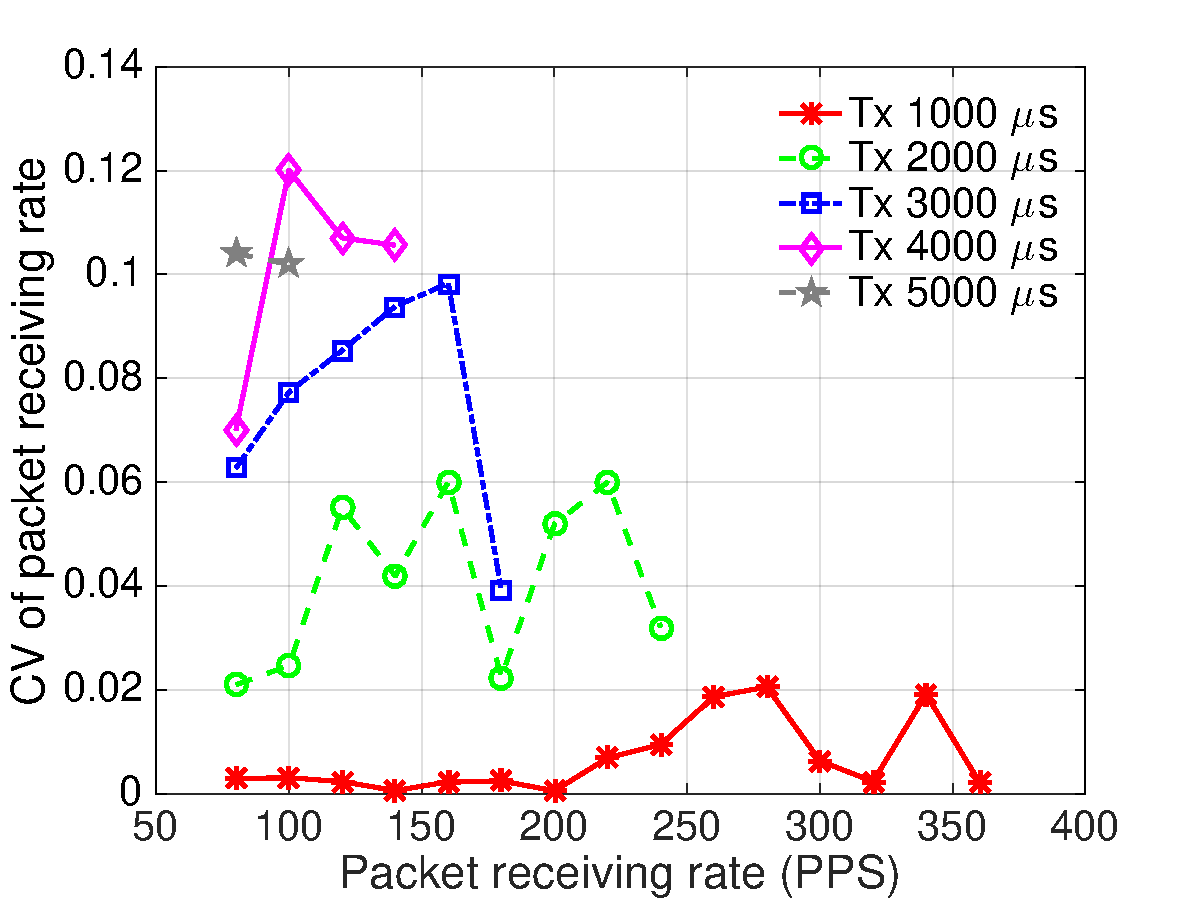
\includegraphics[width=0.45\textwidth]{figures/new_load_avg_result_Prate_tx_all_08_L60}}
  \caption{\gls{cov} of packet receiving rate as a function of packet receiving rate for different average transmission time. 
  %consisting of different coverage and packet size ranges..
  \label{fig:tx-diff-Prate}}
\end{figure*}


\begin{figure}[t]
  \centering
  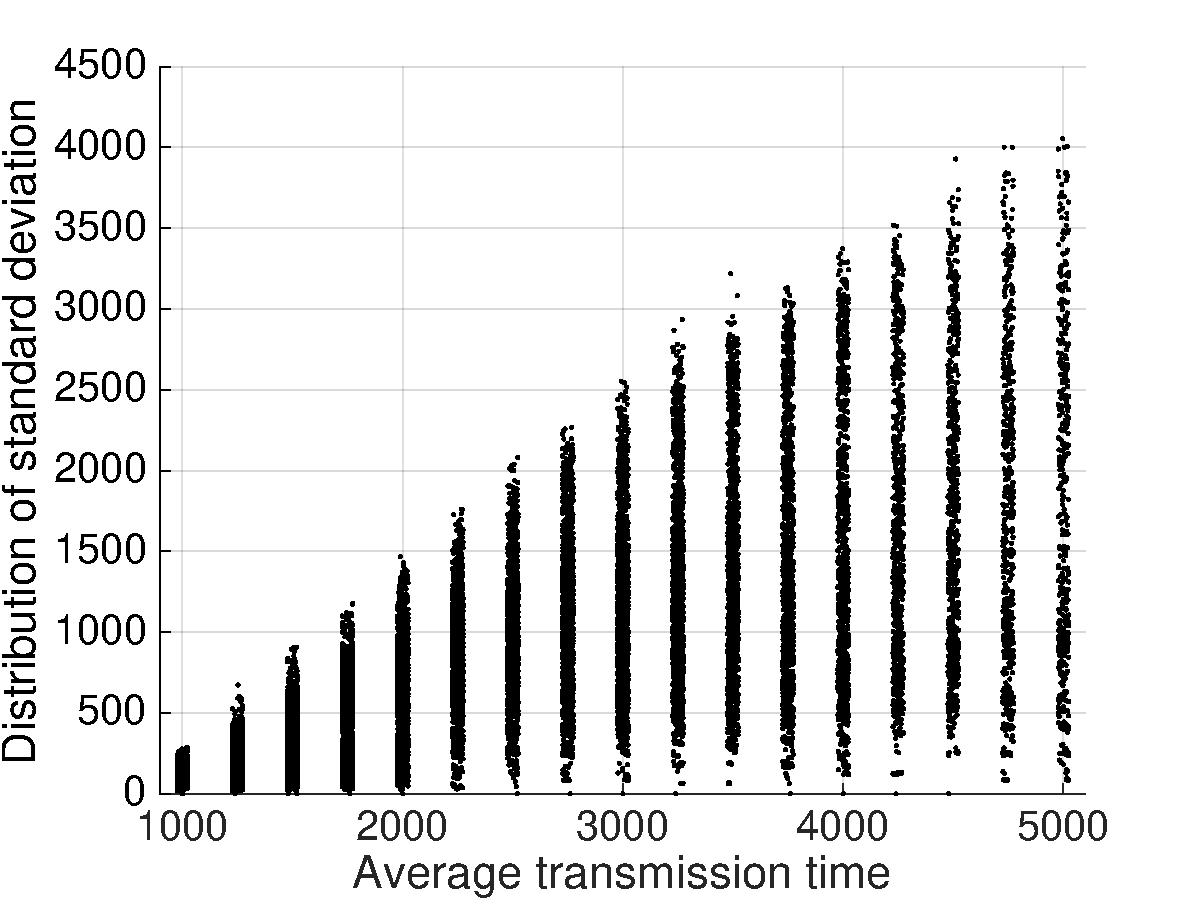
\includegraphics[width=0.85\columnwidth]{figures/std-txtime-distribution}
  \caption{Distribution of standard deviation for different average packet transmission time. \label{fig:tx-std-dist}}
\end{figure}


% \begin{figure}[t]
%   \centering
%   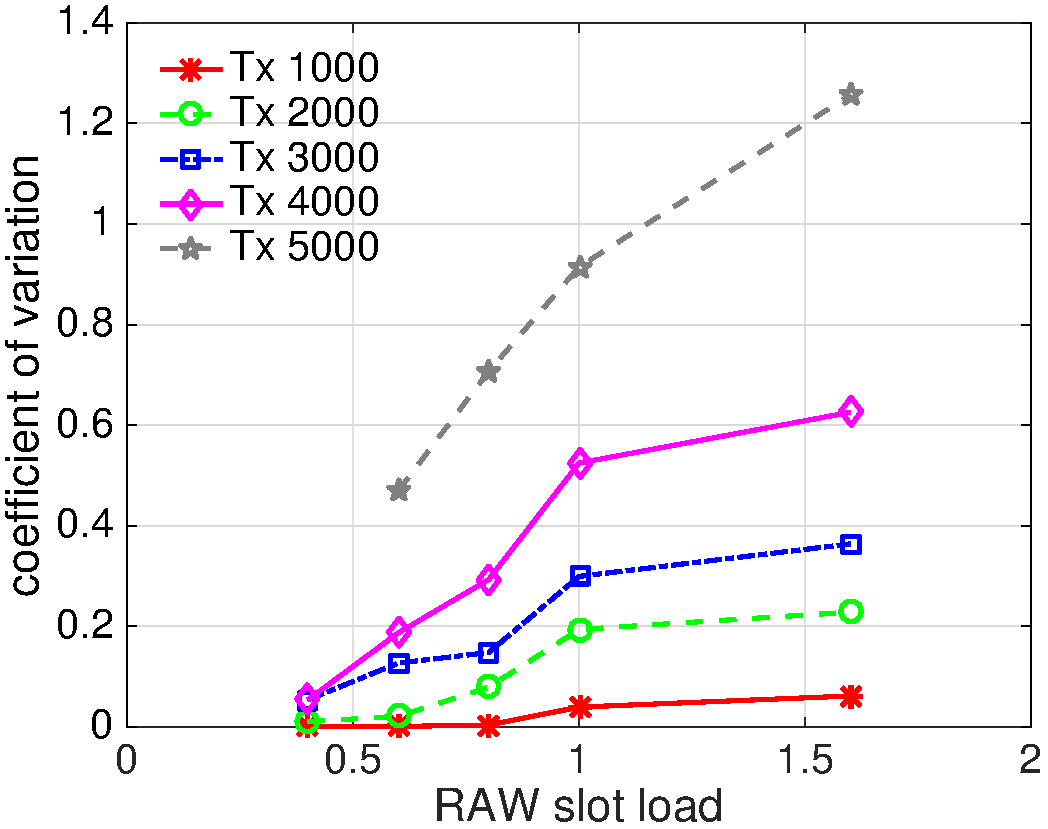
\includegraphics[width=0.75\columnwidth]{figures/result_new_load_cov.pdf}
%     \caption{Coefficient of variation as a function of \gls{raw} slot load rate for each average transmission time consisting of different coverage range and packet size range.
%     \label{fig:tx-diff-load}}
%     % new load ratio 1_8
% \end{figure}

\begin{figure*}[t]
    \centering
    \subfloat[All data points  \label{fig:tx-diff-load-all}]{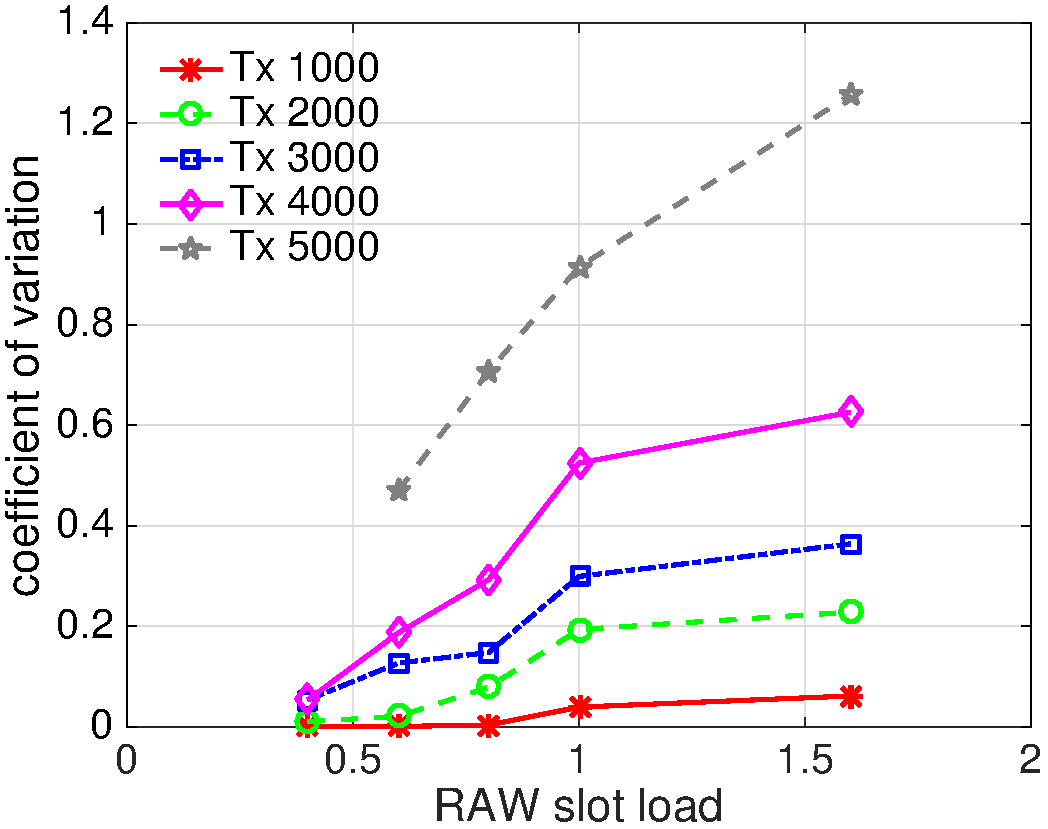
\includegraphics[width=0.45\textwidth]{figures/result_new_load_cov}} 
    \subfloat[data points with \gls{pdr} more than 80\% \label{fig:tx-diff-load-08}]{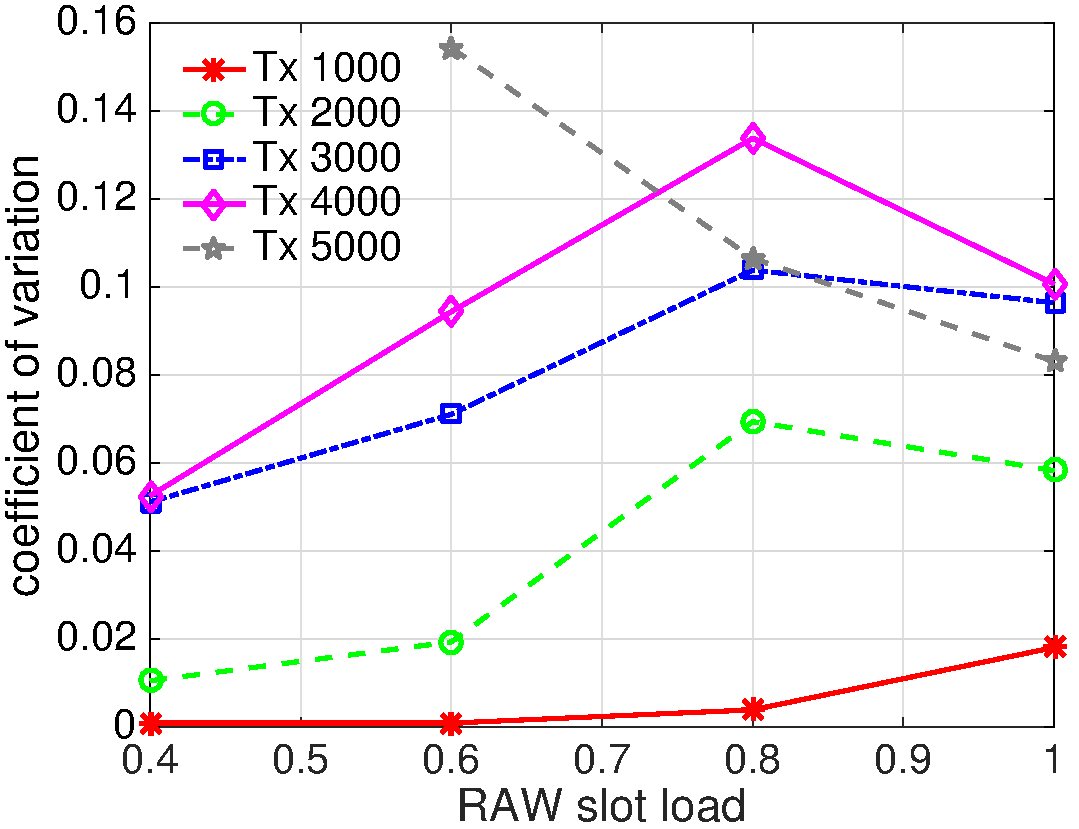
\includegraphics[width=0.45\textwidth]{figures/result_new_load_cov_08}}
  \caption{\gls{cov} as a function of \gls{raw} slot load rate for different average transmission time.
  %consisting of different coverage and packet size ranges..
  \label{fig:tx-diff-load}}
\end{figure*}


% \begin{figure}[t]
%     \centering
%     \subfloat[Tx 1000-4000 us  \label{fig:tx-diff-load}]{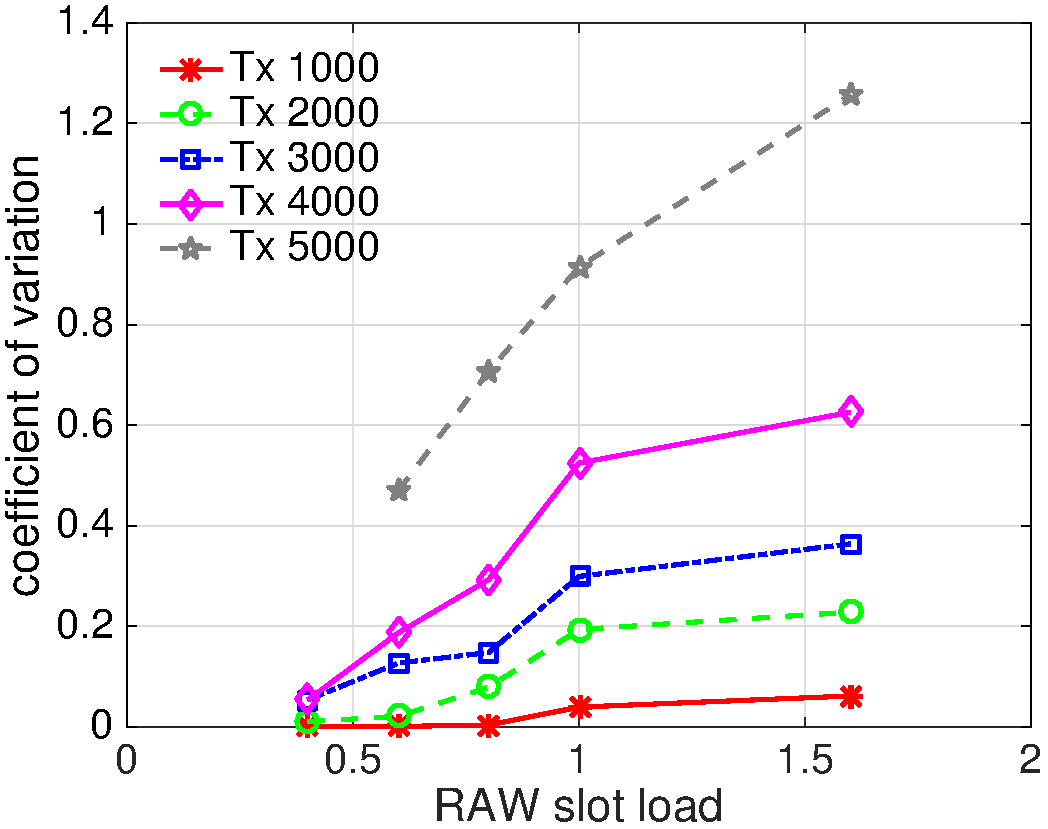
\includegraphics[width=0.8\columnwidth]{figures/result_new_load_cov.pdf}} \\
%     \subfloat[Tx 4000-5000 us  \label{fig:tx-diff-Prate}]{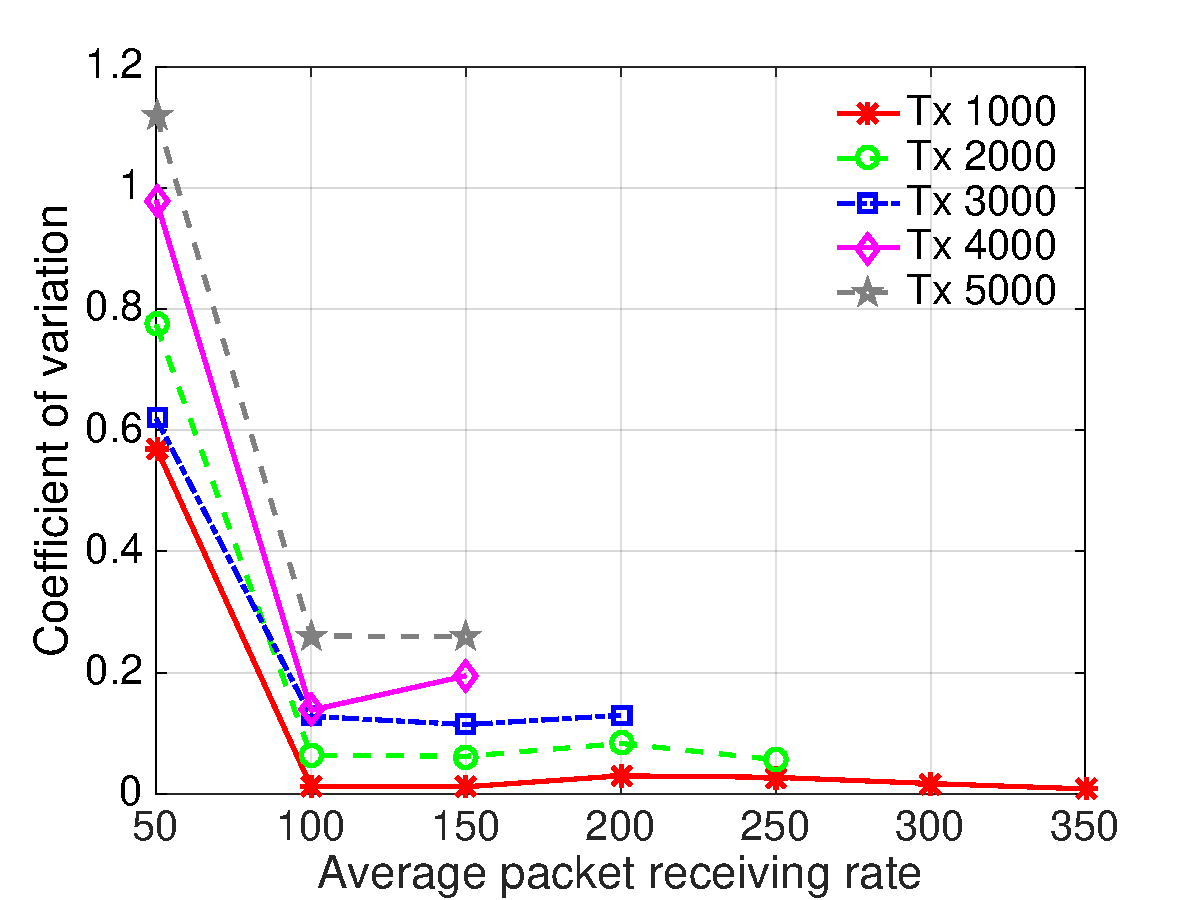
\includegraphics[width=0.8\columnwidth]{figures/new_load_avg_result_Prate_tx.pdf}}
%   \caption{Coefficient of variation as a function of packet receiving rate for each average transmission time consisting of different coverage range and packet size range  \label{fig:tx-diff}}
% \end{figure}



% \begin{figure}
%   \centering
%   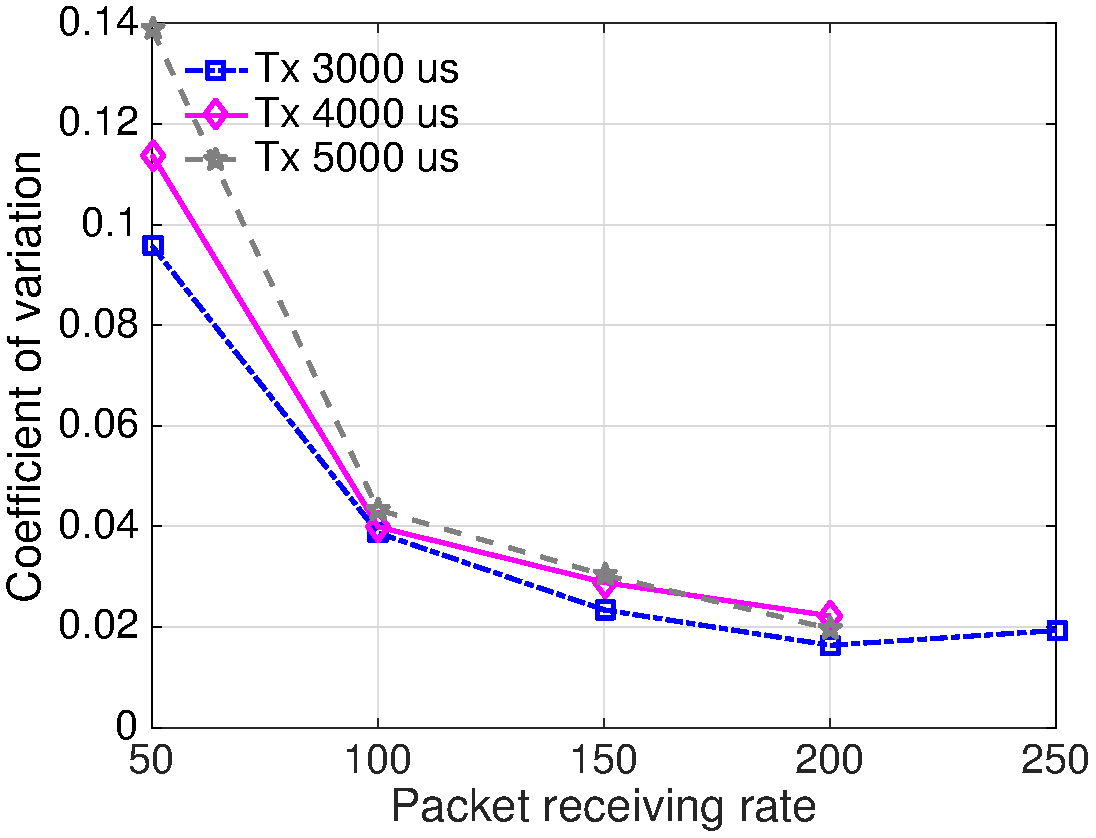
\includegraphics[width=0.75\columnwidth]{figures/avg_result_Prate_tx_ratio3_20_line}
%   \caption{result of different tx time with line. \label{fig:tx-diff-line}}
% \end{figure}


\begin{table}[t]
\centering
\renewcommand{\arraystretch}{1.2}
%\tiny
\caption{\textsc{Definition of the input parameter space}\label{tab:sumo parameters}}
\begin{tabular}{llll}
\hline
\textbf{Parameter}       & \textbf{Min}  & \textbf{Step}   & \textbf{Max}  \\
\hline
$n_r$        & 60 & 5 & 400  \\
$d_r$ ($\mu$s)          & 40960 & 5120 & 204800    \\
$s_r$           & 1 & 5 & 50    \\
$\hat{t}_p$ ($\mu$s)           & 1000 & 250 & 5000    \\
\hline
\end{tabular}
\end{table}


 

% The results in previous section have demonstrated that the created model has quite good accuracy on predicting the output of a given \gls{raw} configuration. In this section, we explore the performance of the model when the average transmission time are generate by  distance and packet size ranges that are not used during the modeling process.

% The variable used by the \gls{raw} modeling, \textit{average transmission time}, is actually represented by two parameters of the 802.11ah network, i.e., distance between stations and \gls{ap}, and packet size of the stations. 



 %\item Training methodology (the evaluation scenario used for training)
\subsection{Training methodology \label{subs:raw_training}}

% Surrogate modeling provides the answer \cite{SUMOtoolbox2010}. 
% A surrogate model is trained at design
% time, using a limited number of input-output sample data
% points obtained through simulation or real-life experiments.
% Surrogate modeling is especially suited for tasks with a large
% input space, as an accurate model can be trained based on
% relatively little input data points. Moreover, evaluating the
% model at runtime is computationally efficient, equivalent to
% a constant-time table lookup. This makes surrogate modeling
% highly suitable for RAW performance modeling, as the input
% space is very large, and efficient runtime model evaluation is
% needed for real-time RAW parameter selection. Additionally,
% by using realistic simulation results, a surrogate model does not suffer from the same restrictive assumptions as existing
% analytical models.

The training of RAW performance surrogate model follows the below steps, using the same numbering as the arrows in Figure \ref{fig:sumo-ns3}:
%When a new sample data point is generated for which the output is unknown, the controller will initiate an ns-3 simulation to determine the output associated with the input parameter values of the data point. 

\begin{enumerate}

\item \label{sm_tr_1} Based on the defined design space (cf. Table~\ref{tab:sumo parameters}), the initial design points are carefully selected to efficiently characterize the system. Each data point has four input parameters, i.e., number of stations, number of slots, \gls{raw} duration, and average transmission time.

%The latin hypercube design (LHD) method is used here to select the design points. It is the most commonly used approach for intial design points selection, selecting sample points evenly along the configuration space while ensuring proportional representation of design variables.

\item \label{sm_tr_2} The ns-3 simulator executes experiments with parameters from each initial data point and the general parameters of 802.11ah (cf. Table~\ref{tab:ns3 parameters}). The evaluation criterion (e.g., packet receiving rate) of the experiments are considered as the output of each data point. 

\item \label{sm_tr_3} After the experiments with all the initial data points, an initial surrogate model is created.

%and calculates the cross validation score. If the score is below the threshold, the experiment stops executing. Otherwise, it continues with the next step.

\item \label{sm_tr_4} The sampling strategy is applied to select the next data points to improve the model accuracy.

\item \label{sm_tr_5} The experiments are executed for the newly selected data points, the evaluation criterion of the experiments is considered as the output of the new data points. 

\item \label{sm_tr_6} The surrogate model is updated with the newly selected data points.

\item \label{sm_tr_7}  This process stops once the stop conditions are met, otherwise it continues with step \ref{sm_tr_4}.
\end{enumerate}


Each experiment in ns-3 runs for 60 seconds of simulated time. As \gls{raw} is configured in each beacon interval of 204.8~ms, the results of every simulated configuration are averaged over 290 beacon intervals, ensuring the generality of the trained model.
The SUMO toolbox is configured to use the proper method in each step in order to create an accurate surrogate model with a limited number of data points. 


\begin{itemize}
\item \textbf{Initial design points selection}  \\
 We use the latin hypercube design (LHD) ~\cite{FAViana2013} approach to select the initial data points, which has the best performance in general and is  most commonly used. It selects sample points evenly along the configuration space while ensuring proportional representation of design variables. Furthermore, the initial sample size depends on the problem type, 200 initial data points was found a good choice for our problem.
 
\item \textbf{The (initial) surrogate model creation}  \\
There are a variety of supervised machine learning and regression methods can be used for surrogate model creation, such as Kriging \cite{forrester2008engineering}, polynomial response surfaces, radial basis functions, support vector machines (SVMs),  space mapping, or artificial neural networks (ANNs). Among these methods, Kriging model is 
very popular in the modeling of  complex systems, including complex wireless network \cite{SUMOWirelessConferencing,wowmom2018, LTEoptimization}.The Kriging model is formed as:
\begin{equation}
\hat{f} (X) = \sum_{i=1}^{V} {a_i}{k(x, x_i)}
\end{equation}
Where $V$ is the amount of basis vectors, $x$ represent the input data vector and $k(x, x_i)$ is the kernel function. There are several kernel (covariance) functions used in kriging, such as Squared Exponential Kernel, Exponential Kernel, Matern 3/2, Matern 5/2, Rational Quadratic Kernel. Among them, the Matern types of kernel functions are  widely used, and we use the Matern kernel function with %$v=3/2$ and 
$5/2$ to create the model. 

\item \textbf{Sampling strategies} \\
A novel sampling strategy called FLOLA-Voronoi \cite{vanderherten2015} is used to select the next design points to improve the model accuracy.  The FLOLA approach is used for exploiting the non-linear regions, while the Voronoi approach explores the sparsely sampled regions, the scores from  the FLOLA and Voronoi are combined to decide the next sample point. In our experiments, 10 new data points are picked in each interation.

% The initial design points explores the configuration space of the system by applying the appropriate design points selection approaches. However, further exploration is needed since the number initial design points is limited, moreover, the initial model may not exploit interesting regions of the system(i.e., non-linear regions).  Therefore, during the sequential design process, at each iteration, the (Root Relative Squared Error (RRSE)  of the currently created surrogate is checked and new sample points is selected if the model accuracy is not satisfactory. 
 


%  As the non-linear regions are difficult to model compared to linear regions, more sample points are required in the modeling process. Therefore, the FLOLA approach uses the local linear approximations to estimate the linearity of the region, with the aim of further exploring these regions. For the Voronoi part, a Voronoi tessellation diagram is drawn from tested points and  the area of each Voronoi cell is calculated. A smaller area indicates the presence of nearby explored data points, representing a tightly explored region. A wider area indicates the absence of nearby points, or a sparsely explored region.  Finally, the scores from the the FLOLA and Voronoi are combined to decide the next sample point.

\item \textbf{Stopping Criteria} \\
%A stop criteria is needed to terminate the modeling process when the intermediary model is accurate enough.
The 10-fold cross-validation with a \gls{rrse} measure is used to evaluate the model accuracy. The modeling process stops once the cross validation score remains stable (3 digits of precision) for 10 successive iterations, i.e., 100 sample data points. Moreover, the stopping criteria are upper limited to a maximum number (i.e., 10000) of iterations and it will stop execution once the iteration number reaches the limit.
% The training stops once the cross
% validation score lower than or equal to 0:10 (2 digits of
% precision) occurs 10 times in succession, or the number of
% training data points exceeds 2500.


% During the modeling process, the accuracy of model is verified by using cross validation method. At each iteration, the previously obtained samples are divided into training and testing sets, and the predicted response of the model built from the training set is compared against the testing set. The modeling process stops once the cross validation score is below a certain level for a certain number of consecutive iterations. Moreover, the stopping criteria are upper limited to a maximum number of iterations and it will stop execution once the iteration number reaches a specified limit.

\end{itemize}






% To obtain a better initial model, the number of initial sample
% points should be large, however, this increase the training time,
% therefore, a trade-off in terms of the initial design points is
% normally made.





%\end{itemize}
